\section{Pianificazione}
\subsection{Introduzione}
In tale sezione, aggiornata progressivamente, sono riportate le descrizioni dei vari periodi e i relativi $\textit{sprint}_G$.
La pianificazione è suddivisa nelle seguenti fasi:
\begin{enumerate}
    \item Studio dei capitolati e assegnazione dell'appalto;
    \item Verso la $\textit{RTB}_G$ (\emph{Requirements and Technology Baseline});
    \item Verso la $\textit{PB}_G$ (\emph{Product Baseline}).
\end{enumerate}
\subsubsection{Preventivi}
In quanto gruppo ad "intensità media", come da "Regolamento del Progetto Didattico" ogni membro del gruppo si impegna a dare la disponibilità per almeno 80 ore produttive. Nelle sezioni seguenti verranno elencati i preventivi relativi alle varie fasi di vita del progetto, con una suddivisione dei ruoli che si è cercata di realizzare nel modo più equo possibile, al fine di dare a tutti i membri la possibilità di approfondire le attività più rilevanti.  
\subsubsection{Consuntivi}
Vengono poi analizzate le risorse che sono state effettivamente impiegate durante le fasi di sviluppo del progetto. L'idea è di rendere immediatamente visibili eventuali scostamenti dal piano originale. \\
L'idea dietro questa analisi è quella di identificare eventuali scostamenti dal piano iniziale e reagire di conseguenza, al fine di apportare un miglioramento continuo. 

\subsection{Studio dei capitolati e assegnazione dell'appalto}
In questa fase preliminare il gruppo, appena formato, discute dei capitolati e si candida per uno di essi. Una volta aggiudicato l'appalto dal prof. Vardanega inizierà la fase successiva ovvero la $\textit{RTB}_G$ (\emph{Requirements and Technology Baseline}).

\begin{table}[h]
\centering
\captionsetup{justification=centering}

\begin{tabular}{|c|c|c|}
\hline
\textbf{Data di inizio} & \textbf{Data di fine prevista} & \textbf{Data di assegnazione dell'appalto} \\
\hline
14/10/2023 & 6/11/2023 & 8/11/2023 \\
\hline
\end{tabular}
\caption{Periodo di studio dei capitolati e assegnazione dell'appalto}
\end{table}

\subsubsection{Attività svolte}
Durante questa fase preliminare, dopo la formazione del gruppo \emph{RAMtastic6}, sono state svolte diverse attività. \\
Inizialmente, sono stati individuati i capitolati di interesse e, dopo varie riunioni interne, si è deciso di presentare la $\textit{candidatura}_G$ per il $\textit{capitolato}_G$ C3, \emph{Easy Meal}. A supporto di questa decisione, è stata creata un'organizzazione omonima al gruppo e un $\textit{repository}_G$ chiamato \emph{Project14} sulla piattaforma \emph{GitHub}. 

Successivamente, è stato organizzato un incontro con \emph{Imola Informatica}, il proponente del $\textit{capitolato}_G$ C3, per discutere dei dettagli.

Inizialmente i dubbi principali che sono emersi riguardavano la definizione degli strumenti da utilizzare, sia a livello di realizzazione ($\textit{tecnologie}_G$ front-end, back-end, database, ecc.), sia a livello organizzativo (versioning, project management).

Nel secondo periodo, che va dal 31 ottobre 2023 al 6 novembre 2023, sono state pianificate e svolte ulteriori attività. In particolare, si è proceduto con la presentazione della $\textit{candidatura}_G$ per il $\textit{capitolato}_G$ C3 - $\textit{Easy Meal}_G$ tramite i relativi documenti. In particolare è stata redatta la seguente documentazione: \emph{"$\textit{Preventivo}_G$ costi e assunzione impegni"}, \emph{"Lettera di presentazione"} e \emph{"Valutazione dei capitolati"}. In ultimo si è effettuato un primo tentativo di organizzazione del lavoro.

Durante questo periodo, la $\textit{candidatura}_G$ è stata valutata dal Prof. Vardanega ed è stata inizialmente rifiutata; tuttavia, dopo varie riunioni interne, sono stati apportati diversi miglioramenti. Il $\textit{repository}_G$ è stato riorganizzato, è stato introdotto un $\textit{sistema}_G$ di $\textit{versionamento}_G$ per i documenti, i documenti della $\textit{candidatura}_G$ sono stati aggiornati, è stato iniziato il documento \emph{"$\textit{Norme di Progetto}_G$"} e sono stati assegnati ruoli specifici a ciascun membro del gruppo. In particolare, è stato modificato il documento di \emph{"Dichiarazione degli impegni"} con la corretta retribuzione oraria.

Nella retrospettiva dopo la valutazione della $\textit{candidatura}_G$ da parte del prof. Vardanega, è emerso il dubbio riguardante uno sbilanciamento tra le ore totali di progettazione (150) e programmazione (126) evidenziato dall'analisi della $\textit{candidatura}_G$. Dopo una discussione interna, il gruppo ha ritenuto necessario che le ore di progettazione siano minori o uguali alle ore di programmazione, inoltre si è notato che le ore del verificatore (120) potrebbero non essere bilanciate.

Dopo il secondo tentativo, la $\textit{candidatura}_G$ è stata approvata e si è potuto procedere con la fase $\textit{RTB}_G$. 
\subsection{Verso la RTB}
La fase $\textit{RTB}_G$ (\emph{Requirements and Technology Baseline}) comprende diversi obiettivi da soddisfare, di seguito elencati:
\begin{itemize}
    \item definire i requisiti, in accordo con il proponente, nel documento \textbf{Analisi dei Requisiti};
    \item dimostrare l'adeguatezza, la compatibilità e la fattibilità delle $\textit{tecnologie}_G$, $\textit{framework}_G$ e librerie scelte tramite il \textbf{PoC}.
\end{itemize}
A supporto di tali attività vi sono altri obblighi documentali:
\begin{itemize}
    \item il presente \textbf{Piano di Progetto};
    \item il \textbf{Piano di Qualifica}:\\
    documento che identifica le metriche e le strategie necessarie per garantire qualità al prodotto finale;
    \item il \textbf{Glossario}:\\
    documento che fornisce definizioni chiare e precise di termini ambigui o ritenuti necessari per comprendere un determinato contesto;
    \item \textbf{Norme di Progetto}:\\
    documento che definisce con precisione le regole che il gruppo dovrà rispettare durante l'arco di svolgimento del progetto;
    \item \textbf{Verbali} interni ed esterni.
\end{itemize}
Ciascuno dei documenti elencati dovrà essere archiviato in un  $\textit{repository}_G$ accessibile dal committente e dal proponente. Ciascuno degli obiettivi sopra elencati ed evidenziati in grassetto corrisponde nel $\textit{software}_G$ di $\textit{versionamento}_G$ \emph{jira} ad un elemento di tipo \emph{"Epic"} utilizzato per raggruppare un insieme di task di minori dimensioni.\\
I periodi presentati in questa sezione saranno descritti tramite le fasi di \emph{sprint planning}, \emph{sprint review} e \emph{sprint retrospective}. In ogni periodo, a partire dall'introduzione di \emph{Jira}, le ore che riguardano il $\textit{preventivo}_G$ e il $\textit{consuntivo}_G$ sono riportate in formato decimale perché rappresentano in modo più' dettagliato le task assegnate.

\newpage
% Primo periodo
% Primo periodo
\subsubsection{Primo periodo (8/11/2023 - 26/11/2023)}

\subsubsubsection{Planning}
\subsubsubsubsection*{Attività pianificate}
All'inizio del periodo ad ogni membro del gruppo sono stati assegnati ruoli specifici, di seguito riportati:
\begin{table}[H]
\centering
\begin{tabular}{|c|c|c|}
\hline
\textbf{Membro} & \textbf{Ruolo} \\
\hline
Samuele V. & Analista \\
\hline
Michele Z. & Verificatore \\
\hline
Leonardo B. & Amministratore \\
\hline
Riccardo Z. & Analista \\
\hline
Filippo T. & Responsabile \\
\hline
Davide B. & Progettista \\
\hline
\end{tabular}
\caption{Ruoli assunti per ciascun membro del team all'inizio del periodo}
\end{table}
\\
Gli obiettivi posti per lo sprint sono stati i seguenti:
\begin{itemize}
    \item Approfondire in collaborazione con il proponente le tecnologie da utilizzare e i requisiti del progetto;
    \item Iniziare il documento di \emph{Analisi dei Requisiti};
    \item Ideare un sistema di versionamento regolamentato per i documenti;
    \item Continuare \emph{Norme di Progetto}.
\end{itemize}

\subsubsubsubsection*{Preventivo}
\begin{table}[H]
    \centering
\begin{spreadtab}{{tabular}{|c|c|c|c|c|c|c|c|}}
    \hline
    @\textbf{Membro} & @\textbf{Re} & @\textbf{Amm} & @\textbf{An} & @\textbf{Progr} & @\textbf{Proge} & @\textbf{Ve} & @\textbf{Totale} \\
    \hline
    @ Samuele V.   & 0          & 0          & 3         & 0          & 0     & 0     & sum(b2:g2) \\
    @ Leonardo B.  & 0         & 1          & 0        & 0        & 0     & 0    & sum(b3:g3) \\
    @ Riccardo Z.  & 0          & 0          & 3          & 0          & 0     & 0   & sum(b4:g4) \\
    @ Davide B.    & 0          & 0          & 0       & 0       & 0     & 3     & sum(b5:g5) \\
    @ Michele Z.   & 0          & 0          & 0         & 0          & 0     & 4     & sum(b6:g6) \\
    @ Filippo T.   & 2          & 0          & 0         & 0          & 0     & 0     & sum(b7:g7) \\
    \hline
    @\textbf{Ore totali} & sum(b2:b7) & sum(c2:c7) & sum(d2:d7) & sum(e2:e7) & sum(f2:f7) & sum(g2:g7) &  sum(b8:g8)\\
    \hline
    @\textbf{Costo totale} & 30*b8 & 20*c8 & 25*d8 & 15*e8 & 25*f8 & 15*g8 & sum(b9:g9)\\
    \hline
\end{spreadtab}
    \caption{Preventivo orario ed economico parziale per il primo periodo, in base al ruolo}
    \label{tab:prev_rtb}
    \vspace{5mm}
    \textbf{Legenda:} \textit{Re} = Responsabile, \textit{Amm} = Amministratore, \textit{An} = Analista, \textit{Progr} = Programmatore, \textit{Proge} = Progettista, \textit{Ve} = Verificatore
\end{table}

\begin{figure}[H]
  \centering
  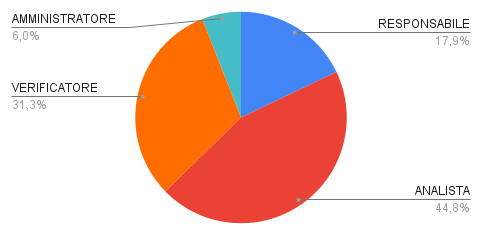
\includegraphics[width=0.6\linewidth]{grafici/1_periodo_torta.png}
  \caption{Ripartizione dei costi per ruolo nel $1^\circ$ periodo}
        \vspace{10mm}
  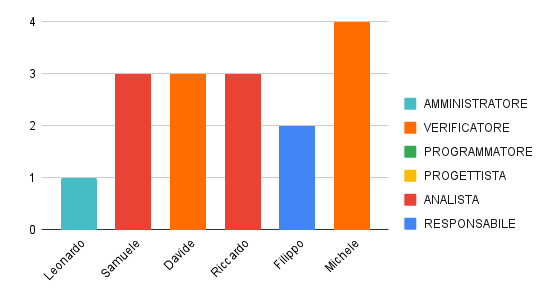
\includegraphics[width=0.7\linewidth]{grafici/1_periodo_istogramma.png}
  \caption{Ore preventivate per ciascuna persona nel $1^\circ$ periodo}
\end{figure}

\subsubsubsection{Review}
\subsubsubsubsection*{Attività svolte}
Le attività preventivate sono state svolte con successo e sono state le seguenti:
\begin{itemize}
    \item E' stato deciso un un workflow per l'utilizzo dei repository di GitHub ovvero \emph{GitFlow};
    \item E' stato elaborato un sistema regolamentato per il versionamento dei documenti;
    \item E' stato modificato il documento di \emph{”Dichiarazione degli impegni”} secondo le indicazioni del prof. Vardanega;
    \item E' continuata la stesura del documento \emph{Norme di Progetto};
    \item Si è deciso di utilizzare \emph{Overleaf} per la stesura dei documenti e solo dopo la verifica il documento verrà caricato nel repository \emph{Project14} tramite file pdf;
    \item E' stata ideata una prima bozza del documento di \emph{Analisi dei Requisiti};
    \item E' stato effettuato un incontro con il proponente durante il quale:
    \begin{itemize}
        \item Si è individuato \emph{React} come probabile libreria da utilizzare;
        \item Sono state fornite risorse e link utili per approfondire gli strumenti il gruppo andrà ad utilizzare;
        \item È stata posta enfasi sull'uso di \emph{Docker} per il deployment;
        \item Si è discusso dei casi d'uso;
        \item Sono stati risolti i dubbi riguardanti il \emph{PoC} e in particolare riguardo alle feature da includere.
    \end{itemize}
\end{itemize}
\subsubsubsubsection*{Consuntivo}
\begin{table}[H]
    \centering
\begin{spreadtab}{{tabular}{|c|c|c|c|c|c|c|c|}}
    \hline
    @\textbf{Membro} & @\textbf{Re} & @\textbf{Amm} & @\textbf{An} & @\textbf{Progr} & @\textbf{Proge} & @\textbf{Ve} & @\textbf{Totale} \\
    \hline
    @ Samuele V.   & 0          & 0          & 3         & 0          & 0     & 0     & sum(b2:g2) \\
    @ Leonardo B.  & 0         & 1          & 0        & 0        & 0     & 0    & sum(b3:g3) \\
    @ Riccardo Z.  & 0          & 0          & 3          & 0          & 0     & 0   & sum(b4:g4) \\
    @ Davide B.    & 0          & 0          & 0       & 0       & 0     & 3     & sum(b5:g5) \\
    @ Michele Z.   & 0          & 0          & 0         & 0          & 0     & 4     & sum(b6:g6) \\
    @ Filippo T.   & 2          & 0          & 0         & 0          & 0     & 0     & sum(b7:g7) \\
    \hline
    @\textbf{Ore totali} & sum(b2:b7) & sum(c2:c7) & sum(d2:d7) & sum(e2:e7) & sum(f2:f7) & sum(g2:g7) &  sum(b8:g8)\\
    \hline
    @\textbf{Costo totale} & 30*b8 & 20*c8 & 25*d8 & 15*e8 & 25*f8 & 15*g8 & sum(b9:g9)\\
    \hline
\end{spreadtab}
    \caption{Consuntivo orario ed economico parziale per il primo periodo, in base al ruolo}
    \label{tab:prev_rtb}
    \vspace{5mm}
    \textbf{Legenda:} \textit{Re} = Responsabile, \textit{Amm} = Amministratore, \textit{An} = Analista, \textit{Progr} = Programmatore, \textit{Proge} = Progettista, \textit{Ve} = Verificatore
\end{table}
\subsubsubsection{Retrospective}
I rischi verificati in questa fase sono stati: \nameref{ro:1}, \nameref{ro:4}.
In questo primo periodo di assestamento ci sono stati diversi dubbi sulla stesura del documento \emph{Piano di Qualifica}, non ancora iniziato. Inoltre, rispetto al documento \emph{Analisi dei Requisiti} non si sono definite delle linee guida utili per il suo sviluppo causando rallentamenti successivi. Inoltre non è risultata chiara la distinzione ore individuali/produttive e, di conseguenza, il loro tracciamento.
%\subsubsubsubsection*{Rischi verificati}

%\subsubsubsubsection*{Analisi retrospettiva}

\newpage
% Secondo periodo
% Secondo periodo
\subsubsection{Secondo periodo (27/11/2023 - 12/12/2023)}

\subsubsubsection{Planning}
\subsubsubsubsection*{Attività pianificate}
All'inizio del periodo ad ogni membro del gruppo sono stati assegnati ruoli specifici, di seguito riportati:
\begin{table}[H]
\centering
\begin{tabular}{|c|c|c|}
\hline
\textbf{Membro} & \textbf{Ruolo} \\
\hline
Samuele V. & Responsabile \\
\hline
Michele Z. & Analista \\
\hline
Leonardo B. & Analista \\
\hline
Riccardo Z. & Programmatore \\
\hline
Filippo T. & Verificatore \\
\hline
Davide B. & Amministratore \\
\hline
\end{tabular}
\caption{Ruoli assunti per ciascun membro del team all'inizio del periodo}
\end{table}
Si è deciso di non coinvolgere il ruolo di "Progettista"  e, invece, di introdurre il ruolo di ”Programmatore” come figura che, almeno nelle prime fasi di vita del progetto, si occuperà della stesura dei verbali e altri documenti.

Gli obiettivi posti per lo sprint sono stati i seguenti:
\begin{itemize}
    \item Approfondire con il proponente le tecnologie da utilizzare;
    \item Cominciare la stesura del documento \emph{Piano di Progetto};
    \item Continuare la stesura del documento \emph{Analisi dei Requisiti};
    \item Approfondire i linguaggi e librerie emersi dall'ultimo incontro con il proponente:
    \begin{itemize}
        \item \emph{Javascript};
        \item \emph{React};
        \item \emph{Docker}.
    \end{itemize}
    \item Approfondire con il proponente alcune questioni emerse sul documento di \emph{Analisi dei Requisiti};
\end{itemize}

\subsubsubsubsection*{Preventivo}
\begin{table}[H]
    \centering
\begin{spreadtab}{{tabular}{|c|c|c|c|c|c|c|c|}}
    \hline
    @\textbf{Membro} & @\textbf{Re} & @\textbf{Amm} & @\textbf{An} & @\textbf{Progr} & @\textbf{Proge} & @\textbf{Ve} & @\textbf{Totale} \\
    \hline
    @ Samuele V.   & 4          & 0          & 0         & 0          & 0     & 1     & sum(b2:g2) \\
    @ Leonardo B.  & 0         & 0          & 3        & 0        & 0     & 0    & sum(b3:g3) \\
    @ Riccardo Z.  & 0          & 0          & 0          & 4          & 0     & 0   & sum(b4:g4) \\
    @ Davide B.    & 0          & 4          & 0       & 0       & 0     & 0     & sum(b5:g5) \\
    @ Michele Z.   & 0          & 0          & 3         & 0          & 0     & 0     & sum(b6:g6) \\
    @ Filippo T.   & 0          & 0          & 0         & 0          & 0     & 4     & sum(b7:g7) \\
    \hline
    @\textbf{Ore totali} & sum(b2:b7) & sum(c2:c7) & sum(d2:d7) & sum(e2:e7) & sum(f2:f7) & sum(g2:g7) &  sum(b8:g8)\\
    \hline
    @\textbf{Costo totale} & 30*b8 & 20*c8 & 25*d8 & 15*e8 & 25*f8 & 15*g8 & sum(b9:g9)\\
    \hline
\end{spreadtab}
    \caption{Preventivo orario ed economico parziale per il secondo periodo, in base al ruolo}
    \label{tab:prev_rtb}
    \vspace{5mm}
    \textbf{Legenda:} \textit{Re} = Responsabile, \textit{Amm} = Amministratore, \textit{An} = Analista, \textit{Progr} = Programmatore, \textit{Proge} = Progettista, \textit{Ve} = Verificatore
\end{table}


\begin{figure}[H]
  \centering
  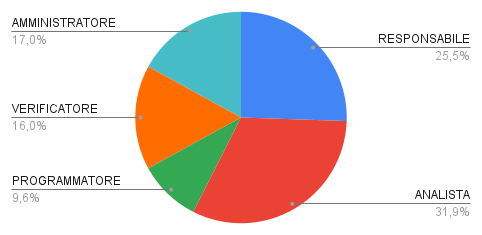
\includegraphics[width=0.6\linewidth]{grafici/2_periodo_torta.png}
  \caption{Ripartizione dei costi per ruolo nel $2^\circ$ periodo}
        \vspace{10mm}
  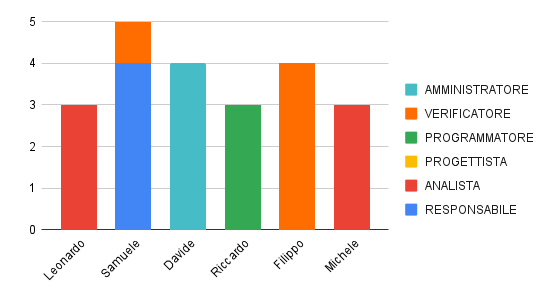
\includegraphics[width=0.7\linewidth]{grafici/2_periodo_istogramma.png}
  \caption{Ore preventivate per ciascuna persona nel $2^\circ$ periodo}
\end{figure}



\subsubsubsection{Review}
\subsubsubsubsection*{Attività svolte}
Le attività preventivate sono state svolte con successo e sono state le seguenti:
\begin{itemize}
    \item E' stato continuato il documento \emph{Analisi Dei Requisiti};
    \item E' stato continuato il documento \emph{Norme di Progetto};
    \item E' stato effettuato dello studio individuale di \emph{Javascript} e \emph{React};
    \item E' stato effettuato un incontro con il proponente durante il quale:
    \begin{itemize}
        \item Sono stati chiariti dubbi sugli scenari secondari di alcuni casi d'uso;
        \item E' stato proposto con successo un timer entro lo scadere del quale è possibile fare le modifiche all'ordinazione collaborativa;
        \item E' stato consigliato l'utilizzo dei framework \emph{Bootstrap} e di \emph{NextJS}.
    \end{itemize}
\end{itemize}
\subsubsubsubsection*{Consuntivo}
\begin{table}[H]
    \centering
\begin{spreadtab}{{tabular}{|c|c|c|c|c|c|c|c|}}
    \hline
    @\textbf{Membro} & @\textbf{Re} & @\textbf{Amm} & @\textbf{An} & @\textbf{Progr} & @\textbf{Proge} & @\textbf{Ve} & @\textbf{Totale} \\
    \hline
    @ Samuele V.   & 3          & 0          & 0         & 0          & 0     & 1     & sum(b2:g2) \\
    @ Leonardo B.  & 0         & 0          & 4        & 0        & 0     & 0    & sum(b3:g3) \\
    @ Riccardo Z.  & 0          & 0          & 0          & 3          & 0     & 0   & sum(b4:g4) \\
    @ Davide B.    & 0          & 3          & 0       & 0       & 0     & 0     & sum(b5:g5) \\
    @ Michele Z.   & 0          & 0          & 3         & 0          & 0     & 0     & sum(b6:g6) \\
    @ Filippo T.   & 0          & 0          & 0         & 0          & 0     & 3     & sum(b7:g7) \\
    \hline
    @\textbf{Ore totali} & sum(b2:b7) & sum(c2:c7) & sum(d2:d7) & sum(e2:e7) & sum(f2:f7) & sum(g2:g7) &  sum(b8:g8)\\
    \hline
    @\textbf{Costo totale} & 30*b8 & 20*c8 & 25*d8 & 15*e8 & 25*f8 & 15*g8 & sum(b9:g9)\\
    \hline
   % @\textbf{Diff. preventivo} & 0 & 0 & 0 & 0 & 0 & 0 & sum(b10:g10)\\
   % \hline
\end{spreadtab}
    \caption{Consuntivo orario ed economico parziale per il secondo periodo, in base al ruolo}
    \label{tab:prev_rtb}
    \vspace{5mm}
    \textbf{Legenda:} \textit{Re} = Responsabile, \textit{Amm} = Amministratore, \textit{An} = Analista, \textit{Progr} = Programmatore, \textit{Proge} = Progettista, \textit{Ve} = Verificatore
\end{table}
\subsubsubsection{Retrospective}

I rischi verificati in questa fase sono stati:\nameref{ro:1},\nameref{ro:4}.
Dal punto di vista organizzativo ci sono stati diversi problemi. Inoltre sono emersi diversi dubbi riguardanti la stesura del documento di \emph{Analisi dei Requisiti}.
In particolare, sono sorti durante l'uso degli USE CASE. Infine ci sono stati dei dubbi riguardo la verifica dello stato di avanzamento dei lavori e su come individuare in quali ambiti si stanno riscontrando criticità.
In particolare sono emerse le seguenti criticità:
\begin{itemize}
    \item Lo scarso utilizzo fino al quel momento di scenari secondari;
    \item Dubbi sulla gestione di eventuali scenari che potrebbero riguardare casi d’uso principali o sotto casi;
    \item Dubbi riguardanti casi d’uso che coinvolgono più attori contemporaneamente;
    \item Dubbi riguardanti l'utilizzo della locuzione \emph{extend}.
\end{itemize}
Per mitigare tali problemi si è ideato un documento interno che riguarda i pattern da seguire per stilare il documento di Analisi dei Requisiti.
\newpage
% Terzo periodo
\subsubsection{Terzo periodo (13/12/2023 - 6/1/2024)}
\subsubsubsection{Planning}
\subsubsubsubsection*{Attività pianificate}
All'inizio del periodo ad ogni membro del gruppo sono stati assegnati ruoli specifici, di seguito riportati:
\begin{table}[H]
\centering
\begin{tabular}{|c|c|c|}
\hline
\textbf{Membro} & \textbf{Ruolo} \\
\hline
Samuele V. & Programmatore \\
\hline
Michele Z. & Analista \\
\hline
Leonardo B. & Programmatore \\
\hline
Riccardo Z. & Analista \\
\hline
Filippo T. & Responsabile \\
\hline
Davide B. & Verificatore \\
\hline
\end{tabular}
\caption{Ruoli assunti per ciascun membro del team all'inizio del periodo}
\end{table}


Gli obiettivi posti per lo $\textit{sprint}_G$ sono stati i seguenti:
\begin{itemize}
    \item Ultimare lo studio dello $\textit{tecnologie}_G$, in particolare approfondire \emph{NextJS};
    \item Continuare la stesura del documento \emph{Analisi dei Requisiti} (in particolare dei casi d'uso);
    \item Iniziare a sviluppare il \emph{PoC} utilizzando le $\textit{tecnologie}_G$ scelte;
    \item Iniziare la stesura di \emph{Piano di Progetto};
    \item Creare una prima bozza del glossario tecnico;
    \item Organizzare seminari con Imola informatica;
    \item Effettuare un incontro con il prof. Cardin.
\end{itemize} 

\subsubsubsubsection*{Preventivo}
\begin{table}[H]
    \centering
\begin{spreadtab}{{tabular}{|c|c|c|c|c|c|c|c|}}
    \hline
    @\textbf{Membro} & @\textbf{Re} & @\textbf{Amm} & @\textbf{An} & @\textbf{Progr} & @\textbf{Proge} & @\textbf{Ve} & @\textbf{Totale} \\
    \hline
    @ Samuele V.   & 0          & 0          & 0         & 3          & 0     & 0     & sum(b2:g2) \\
    @ Leonardo B.  & 0         & 0          & 0        & 4        & 0     & 0    & sum(b3:g3) \\
    @ Riccardo Z.  & 0          & 0          & 5          & 0          & 0     & 0   & sum(b4:g4) \\
    @ Davide B.    & 0          & 0          & 0       & 0       & 0     & 4     & sum(b5:g5) \\
    @ Michele Z.   & 0          & 0          & 4.5         & 0          & 0     & 0     & sum(b6:g6) \\
    @ Filippo T.   & 4          & 0          & 0         & 0          & 0     & 0     & sum(b7:g7) \\
    \hline
    @\textbf{Ore totali} & sum(b2:b7) & sum(c2:c7) & sum(d2:d7) & sum(e2:e7) & sum(f2:f7) & sum(g2:g7) &  sum(b8:g8)\\
    \hline
    @\textbf{Costo totale} & 30*b8 & 20*c8 & 25*d8 & 15*e8 & 25*f8 & 15*g8 & sum(b9:g9)\\
    \hline
\end{spreadtab}
    \caption{Preventivo orario ed economico parziale per il terzo periodo, in base al ruolo}
    \label{tab:prev_rtb}
    \vspace{5mm}
    \textbf{Legenda:} \textit{Re} = Responsabile, \textit{Amm} = Amministratore, \textit{An} = Analista, \textit{Progr} = Programmatore, \textit{Proge} = Progettista, \textit{Ve} = Verificatore
\end{table}

\begin{figure}[H]
  \centering
  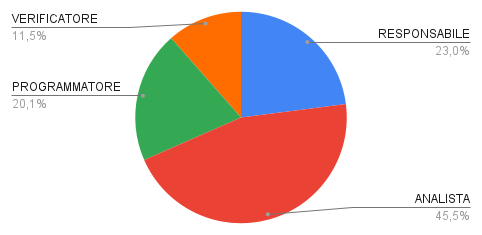
\includegraphics[width=0.6\linewidth]{grafici/3_periodo_torta.png}
  \caption{Ripartizione dei costi per ruolo nel $3^\circ$ periodo}
        \vspace{10mm}
  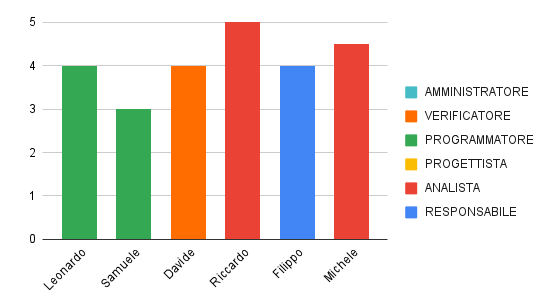
\includegraphics[width=0.7\linewidth]{grafici/3_periodo_istogramma.png}
  \caption{Ore preventivate per ciascuna persona nel $3^\circ$ periodo}
\end{figure}

\subsubsubsection{Review}
\subsubsubsubsection*{Attività svolte}
Le attività preventivate sono state svolte con successo e sono state le seguenti:
\begin{itemize}
    \item E' continuata la stesura del documento di \emph{Analisi dei Requisiti} e \emph{Piano di Progetto};
    \item E' continuato lo studio individuale delle $\textit{tecnologie}_G$ da utilizzare;
    \item E' stato effettuato con il prof. Cardin un incontro per risolvere i dubbi riguardo il documento \emph{Analisi dei Requisiti}, in particolare:
    \begin{itemize}
        \item E' stata chiarita la profondità di dettaglio per specificare ogni $\textit{caso d'uso}_G$;
        \item E' stato fornito un $\textit{feedback}_G$ positivo per quanto riguarda i sotto casi d'uso di \emph{Modifica del menu' di un ristorante};
        \item E' stato chiarito l'utilizzo degli scenari alternativi;
        \item E' stato chiarito che non fosse corretto l'utilizzo di \emph{Database} come $\textit{attore}_G$ secondario.
    \end{itemize}
    \item "Big Bang" dal punto di vista organizzativo, il quale è andato ad impattare sia l'\emph{Analisi de Requisiti} che il \emph{PoC};
\end{itemize}
\subsubsubsubsection*{Consuntivo}
\begin{table}[H]
    \centering
\begin{spreadtab}{{tabular}{|c|c|c|c|c|c|c|c|}}
    \hline
    @\textbf{Membro} & @\textbf{Re} & @\textbf{Amm} & @\textbf{An} & @\textbf{Progr} & @\textbf{Proge} & @\textbf{Ve} & @\textbf{Totale} \\
    \hline
    @ Samuele V.   & 0          & 0          & 0         & 2          & 0     & 0     & sum(b2:g2) \\
    @ Leonardo B.  & 0         & 0          & 0        & 3        & 0     & 0    & sum(b3:g3) \\
    @ Riccardo Z.  & 0          & 0          & 5          & 0          & 0     & 0   & sum(b4:g4) \\
    @ Davide B.    & 0          & 0          & 0       & 0       & 0     & 3     & sum(b5:g5) \\
    @ Michele Z.   & 0          & 0          & 5         & 0          & 0     & 0     & sum(b6:g6) \\
    @ Filippo T.   & 6          & 0          & 0         & 0          & 0     & 0     & sum(b7:g7) \\
    \hline
    @\textbf{Ore totali} & sum(b2:b7) & sum(c2:c7) & sum(d2:d7) & sum(e2:e7) & sum(f2:f7) & sum(g2:g7) &  sum(b8:g8)\\
    \hline
    @\textbf{Costo totale} & 30*b8 & 20*c8 & 25*d8 & 15*e8 & 25*f8 & 15*g8 & sum(b9:g9)\\
    \hline
  %  @\textbf{Diff. preventivo} & 0 & 0 & 0 & 0 & 0 & 0 & sum(b10:g10)\\
  %  \hline
\end{spreadtab}
    \caption{Consuntivo orario ed economico parziale per il terzo periodo, in base al ruolo}
    \label{tab:prev_rtb}
    \vspace{5mm}
    \textbf{Legenda:} \textit{Re} = Responsabile, \textit{Amm} = Amministratore, \textit{An} = Analista, \textit{Progr} = Programmatore, \textit{Proge} = Progettista, \textit{Ve} = Verificatore
\end{table}
\subsubsubsection{Retrospective}
I $\textit{rischi}_G$ verificati in questa fase sono stati: \nameref{rt:1}, \nameref{ro:4}.
Quasi del tutto risolti i problemi dal punto di vista organizzativo, e inoltre il gruppo si sta mettendo in moto per cercare di integrare conoscenze sulle $\textit{tecnologie}_G$ da usare in futuro nel progetto.
 \\
I dubbi principali sono sorti durante l'uso degli USE CASE per stilare il documento di $\textit{analisi dei requisiti}_G$. Inoltre vi sono state difficoltà nell'iniziare lo sviluppo del del \emph{PoC} in quanto non tutti i membri del gruppo sono familiari con l'uso di $\textit{framework}_G$ per lo sviluppo.
Oltre a ciò sono state rilevate diverse difficoltà organizzative, in particolare:
\begin{itemize}
    \item Come gestire in modo ottimale il tempo;
    \item Assenza di obiettivi ben definiti per ogni membro del gruppo.
\end{itemize}
Per mitigare tali problemi attualmente si sta cercando un supporto per rendere quanto più preciso e chiaro possibile il conteggio delle ore.
\newpage
% Quarto periodo
\subsubsection{Quarto periodo (7/1/2024 - 15/1/2024)}
\subsubsubsection{Planning}
\subsubsubsubsection*{Attività pianificate}
All'inizio del periodo ad ogni membro del gruppo sono stati assegnati ruoli specifici, di seguito riportati:
\begin{table}[H]
\centering
\begin{tabular}{|c|c|c|}
\hline
\textbf{Membro} & \textbf{Ruolo} \\
\hline
Samuele V. & Analista \\
\hline
Michele Z. & Amministratore \\
\hline
Leonardo B. & Responsabile \\
\hline
Riccardo Z. & Programmatore \\
\hline
Filippo T. & Verificatore \\
\hline
Davide B. & Analista \\
\hline
\end{tabular}
\caption{Ruoli assunti per ciascun membro del team all'inizio del periodo}
\end{table}


Gli obiettivi posti per lo $\textit{sprint}_G$ sono stati i seguenti:
\begin{itemize}
    \item Delineare una prima versione del \emph{Piano di Progetto};
    \item Continuare ad aggiornare il documento \emph{Norme di progetto};
    \item Iniziare a sviluppare il \emph{PoC}; 
    \item Continuare la stesura di \emph{Analisi dei Requisiti};
    \item Normare in modo più dettagliato i $\textit{processi organizzativi}_G$;
    \item Richiedere un incontro con il proponente per discutere dei requisiti funzionali trovati mediante i casi d'uso;
    \item Iniziare la stesura del glossario tecnico.
\end{itemize}
\subsubsubsubsection*{Preventivo}
\begin{table}[H]
    \centering
\begin{spreadtab}{{tabular}{|c|c|c|c|c|c|c|c|}}
    \hline
    @\textbf{Membro} & @\textbf{Re} & @\textbf{Amm} & @\textbf{An} & @\textbf{Progr} & @\textbf{Proge} & @\textbf{Ve} & @\textbf{Totale} \\
    \hline
    @ Samuele V.   & 0          & 0          & 4         & 0          & 0     & 0     & sum(b2:g2) \\
    @ Leonardo B.  & 2         & 0          & 0        & 0        & 0     & 2    & sum(b3:g3) \\
    @ Riccardo Z.  & 0          & 0          & 0          & 4          & 0     & 0   & sum(b4:g4) \\
    @ Davide B.    & 0          & 0          & 5       & 0       & 0     & 0     & sum(b5:g5) \\
    @ Michele Z.   & 0          & 4          & 0         & 0          & 0     & 0     & sum(b6:g6) \\
    @ Filippo T.   & 0          & 0          & 0         & 0          & 0     & 3     & sum(b7:g7) \\
    \hline
    @\textbf{Ore totali} & sum(b2:b7) & sum(c2:c7) & sum(d2:d7) & sum(e2:e7) & sum(f2:f7) & sum(g2:g7) &  sum(b8:g8)\\
    \hline
    @\textbf{Costo totale} & 30*b8 & 20*c8 & 25*d8 & 15*e8 & 25*f8 & 15*g8 & sum(b9:g9)\\
    \hline
\end{spreadtab}
    \caption{Preventivo orario ed economico parziale per il quarto periodo, in base al ruolo}
    \label{tab:prev_rtb}
    \vspace{5mm}
    \textbf{Legenda:} \textit{Re} = Responsabile, \textit{Amm} = Amministratore, \textit{An} = Analista, \textit{Progr} = Programmatore, \textit{Proge} = Progettista, \textit{Ve} = Verificatore
\end{table}

\begin{figure}[H]
  \centering
  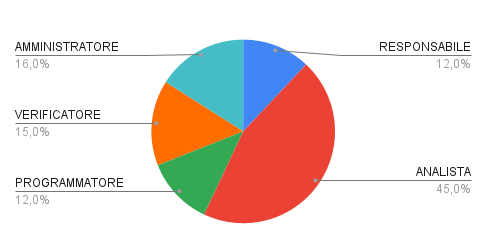
\includegraphics[width=0.6\linewidth]{grafici/4_periodo_torta.png}
  \caption{Ripartizione dei costi per ruolo nel $4^\circ$ periodo}
        \vspace{10mm}
  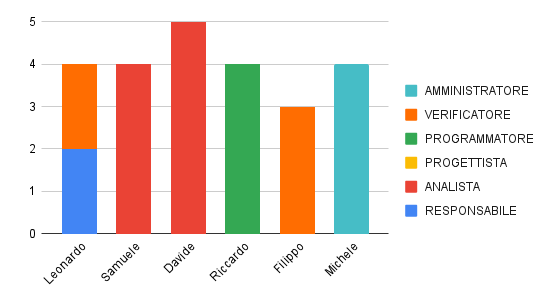
\includegraphics[width=0.7\linewidth]{grafici/4_periodo_istogramma.png}
  \caption{Ore preventivate per ciascuna persona nel $4^\circ$ periodo}
\end{figure}


\subsubsubsection{Review}
\subsubsubsubsection*{Attività svolte}
Periodo di assestamento causa sessione di esami.
Sono state prese le seguenti decisioni:
\begin{itemize}
    \item Utilizzo del $\textit{software}_G$ \emph{Jira} per assegnare le issues e tenere conto del tracciamento temporale di ognuna di esse;
    \item Utilizzo del modello di sviluppo \emph{Scrum};
    \item Utilizzo di linee guida per il documento di \emph{Analisi dei Requisiti} in merito allo stile da adottare nell'uso dei diagrammi e nella specifica testuale dei casi d'uso.
\end{itemize}
\subsubsubsubsection*{Consuntivo}
\begin{table}[H]
    \centering
\begin{spreadtab}{{tabular}{|c|c|c|c|c|c|c|c|}}
    \hline
    @\textbf{Membro} & @\textbf{Re} & @\textbf{Amm} & @\textbf{An} & @\textbf{Progr} & @\textbf{Proge} & @\textbf{Ve} & @\textbf{Totale} \\
    \hline
    @ Samuele V.   & 0          & 0          & 3         & 0          & 0     & 0     & sum(b2:g2) \\
    @ Leonardo B.  & 1.25         & 0          & 1.5        & 0        & 0     & 2    & sum(b3:g3) \\
    @ Riccardo Z.  & 0          & 0          & 0          & 3.5          & 0     & 0   & sum(b4:g4) \\
    @ Davide B.    & 0          & 0          & 3.5       & 0       & 0     & 0     & sum(b5:g5) \\
    @ Michele Z.   & 0          & 3        & 0         & 0          & 0     & 0     & sum(b6:g6) \\
    @ Filippo T.   & 0          & 0          & 0         & 0          & 0     & 3     & sum(b7:g7) \\
    \hline
    @\textbf{Ore totali} & sum(b2:b7) & sum(c2:c7) & sum(d2:d7) & sum(e2:e7) & sum(f2:f7) & sum(g2:g7) &  sum(b8:g8)\\
    \hline
    @\textbf{Costo totale} & 30*b8 & 20*c8 & 25*d8 & 15*e8 & 25*f8 & 15*g8 & sum(b9:g9)\\
    \hline
    %@\textbf{Diff. preventivo} & 0 & -1 & -7 & 0 & 0 & 0 & sum(b10:g10)\\
    %\hline
\end{spreadtab}
    \caption{Preventivo orario ed economico parziale per il quarto periodo, in base al ruolo}
    \label{tab:prev_rtb}
    \vspace{5mm}
    \textbf{Legenda:} \textit{Re} = Responsabile, \textit{Amm} = Amministratore, \textit{An} = Analista, \textit{Progr} = Programmatore, \textit{Proge} = Progettista, \textit{Ve} = Verificatore
\end{table}
\subsubsubsection{Retrospective}
\subsubsubsubsection*{Rischi verificati}
I $\textit{rischi}_G$ riscontrati in questa fase sono stati: \nameref{ro:3},\nameref{ro:4}
Ci sono stati rallentamenti nell'avanzamento dei lavori e difficoltà nel coordinamento delle attività causa l'imminente sessione d'esame. Sono stati risolti, almeno parzialmente, i problemi di tracciamento delle ore tramite l'uso dello $\textit{strumento}_G$ \emph{Jira}.
\newpage
% Quinto periodo
\subsubsection{Quinto periodo (16/1/2024 - 12/2/2024)}
\subsubsubsection{Planning}
\subsubsubsubsection*{Attività pianificate}
Nel corso dello sprint, il team \emph{RAMtastic6} ha previsto un periodo di sospensione parziale delle attività di circa due settimane, dal 22/1/2024 fino al 5/2/2024.
Gli obiettivi posti per lo sprint sono stati i seguenti:
\begin{itemize}
    \item Implementare una prima versione di ricerca e prenotazione del ristorante all'interno del Poc;
    \item Completare il documento \emph{Analisi dei Requisiti} aggiungendo i requisiti funzionali.
\end{itemize}

\subsubsubsubsection*{Preventivo}
\begin{table}[H]
    \centering
\begin{spreadtab}{{tabular}{|c|c|c|c|c|c|c|c|}}
    \hline
    @\textbf{Membro} & @\textbf{Re} & @\textbf{Amm} & @\textbf{An} & @\textbf{Progr} & @\textbf{Proge} & @\textbf{Ve} & @\textbf{Totale} \\
    \hline
    @ Samuele V.   & 0          & 0          & 3         & 0          & 0     & 0     & sum(b2:g2) \\
    @ Leonardo B.  & 4         & 0          & 0        & 0        & 0     & 0.5   & sum(b3:g3) \\
    @ Riccardo Z.  & 0          & 0          & 0          & 5.5          & 0     & 0   & sum(b4:g4) \\
    @ Davide B.    & 0          & 0          & 4       & 0       & 0     & 0     & sum(b5:g5) \\
    @ Michele Z.   & 0          & 2          & 0         & 0          & 0     & 0     & sum(b6:g6) \\
    @ Filippo T.   & 0          & 0          & 0         & 0          & 0     & 4     & sum(b7:g7) \\
    \hline
    @\textbf{Ore totali} & sum(b2:b7) & sum(c2:c7) & sum(d2:d7) & sum(e2:e7) & sum(f2:f7) & sum(g2:g7) &  sum(b8:g8)\\
    \hline
    @\textbf{Costo totale} & 30*b8 & 20*c8 & 25*d8 & 15*e8 & 25*f8 & 15*g8 & sum(b9:g9)\\
    \hline
\end{spreadtab}
    \caption{Preventivo orario ed economico parziale per il quinto periodo, in base al ruolo}
    \label{tab:prev_rtb}
    \vspace{5mm}
    \textbf{Legenda:} \textit{Re} = Responsabile, \textit{Amm} = Amministratore, \textit{An} = Analista, \textit{Progr} = Programmatore, \textit{Proge} = Progettista, \textit{Ve} = Verificatore
\end{table}
\begin{figure}[H]
  \centering
  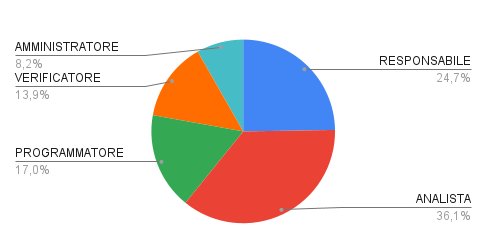
\includegraphics[width=0.6\linewidth]{grafici/5_periodo_torta.png}
  \caption{Ripartizione dei costi per ruolo nel $5^\circ$ periodo}
        \vspace{10mm}
  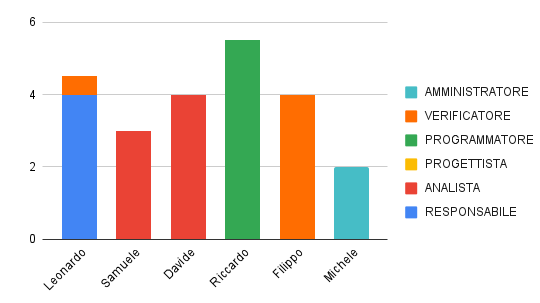
\includegraphics[width=0.7\linewidth]{grafici/5_periodo_istogramma.png}
  \caption{Ore preventivate per ciascuna persona nel $5^\circ$ periodo}
\end{figure}
\subsubsubsection{Review}
\subsubsubsubsection*{Attività svolte}
Per quanto riguarda l'Analisi dei Requisiti:
\begin{itemize}
    \item Sono state apportate correzioni a degli UC esistenti;
    \item Si è creata la sezione requisiti funzionali nel documento \emph{Analisi dei Requisiti}.
\end{itemize} 
\subsubsubsubsection*{Consuntivo}
\begin{table}[H]
    \centering
\begin{spreadtab}{{tabular}{|c|c|c|c|c|c|c|c|}}
    \hline
    @\textbf{Membro} & @\textbf{Re} & @\textbf{Amm} & @\textbf{An} & @\textbf{Progr} & @\textbf{Proge} & @\textbf{Ve} & @\textbf{Totale} \\
    \hline
    @ Samuele V.   & 0          & 0          & 3.75         & 0          & 0     & 0     & sum(b2:g2) \\
    @ Leonardo B.  & 3.25         & 0          & 0        & 0        & 0     & 0.75    & sum(b3:g3) \\
    @ Riccardo Z.  & 0          & 0          & 0          & 5.75          & 0     & 0   & sum(b4:g4) \\
    @ Davide B.    & 0          & 0          & 4.5       & 0       & 0     & 0     & sum(b5:g5) \\
    @ Michele Z.   & 0          & 1.17          & 0         & 0          & 0     & 0     & sum(b6:g6) \\
    @ Filippo T.   & 0          & 0          & 0         & 0          & 0     & 2.42     & sum(b7:g7) \\
    \hline
    @\textbf{Ore totali} & sum(b2:b7) & sum(c2:c7) & sum(d2:d7) & sum(e2:e7) & sum(f2:f7) & sum(g2:g7) &  sum(b8:g8)\\
    \hline
    @\textbf{Costo totale} & 30*b8 & 20*c8 & 25*d8 & 15*e8 & 25*f8 & 15*g8 & sum(b9:g9)\\
    \hline
    %@\textbf{Diff. preventivo} & 0 & 0 & 0 & 1 & 0 & 0 & sum(b10:g10)\\
    %\hline
\end{spreadtab}
    \caption{Consuntivo orario ed economico parziale per il quinto periodo, in base al ruolo}
    \label{tab:prev_rtb}
    \vspace{5mm}
    \textbf{Legenda:} \textit{Re} = Responsabile, \textit{Amm} = Amministratore, \textit{An} = Analista, \textit{Progr} = Programmatore, \textit{Proge} = Progettista, \textit{Ve} = Verificatore
\end{table}
\subsubsubsection{Retrospective}
In questo periodo sono state riscontrate delle problematiche nello sviluppo dei casi d'uso; in particolare è stata rivista la gerarchia degli attori e si è cercato di dare un senso atomico al loro nome. Inoltre, si è riscontrato il rischio \nameref{ro:3} in quanto diversi membri del gruppo erano impegnati con la sessione d'esame. 



\newpage
% Sesto periodo
\subsubsection{Sesto periodo (2024/02/13 - 2024/03/06)}
\subsubsubsection{Planning}
\subsubsubsubsection*{Attività pianificate}
All'inizio del periodo ad ogni membro del gruppo sono stati assegnati ruoli specifici, di seguito riportati:
\begin{table}[H]
\centering
\begin{tabular}{|c|c|c|}
\hline
\textbf{Membro} & \textbf{Ruolo} \\
\hline
Samuele V. & Analista \\
\hline
Michele Z. & Responsabile \\
\hline
Leonardo B. & Amministratore \\
\hline
Riccardo Z. & Analista \\
\hline
Filippo T. & Verificatore \\
\hline
Davide B. & Analista \\
\hline
\end{tabular}
\caption{Ruoli assunti per ciascun membro del team all'inizio del periodo}
\end{table}

Gli obiettivi posti per lo $\textit{sprint}_G$ sono stati i seguenti:
\begin{itemize}
    \item Ultimare gli ultimi \emph{UC} e il documento di \emph{Analisi dei Requisiti};
    \item Iniziare a redigere il glossario tecnico e implementare un'insieme di automazioni utili alla sua costruzione automatica;
    \item Riprendere lo sviluppo del \emph{PoC}.
\end{itemize}


\subsubsubsubsection*{Preventivo}
\begin{table}[H]
    \centering
\begin{spreadtab}{{tabular}{|c|c|c|c|c|c|c|c|}}
    \hline
    @\textbf{Membro} & @\textbf{Re} & @\textbf{Amm} & @\textbf{An} & @\textbf{Progr} & @\textbf{Proge} & @\textbf{Ve} & @\textbf{Totale} \\
    \hline
    @ Samuele V.   & 0          & 0          & 8         & 0          & 0     & 0     & sum(b2:g2) \\
    @ Leonardo B.  & 0         & 3          & 0        & 2.5        & 0     & 0    & sum(b3:g3) \\
    @ Riccardo Z.  & 0          & 0          & 8.5          & 0          & 0     & 0   & sum(b4:g4) \\
    @ Davide B.    & 0          & 0          & 8       & 1.5       & 0     & 0     & sum(b5:g5) \\
    @ Michele Z.   & 5          & 0          & 0         & 0          & 0     & 0     & sum(b6:g6) \\
    @ Filippo T.   & 0          & 0          & 0         & 0          & 0     & 4.5     & sum(b7:g7) \\
    \hline
    @\textbf{Ore totali} & sum(b2:b7) & sum(c2:c7) & sum(d2:d7) & sum(e2:e7) & sum(f2:f7) & sum(g2:g7) &  sum(b8:g8)\\
    \hline
    @\textbf{Costo totale} & 30*b8 & 20*c8 & 25*d8 & 15*e8 & 25*f8 & 15*g8 & sum(b9:g9)\\
    \hline
\end{spreadtab}
    \caption{Preventivo orario ed economico parziale per il sesto periodo, in base al ruolo}
    \label{tab:prev_rtb}
    \vspace{5mm}
    \textbf{Legenda:} \textit{Re} = Responsabile, \textit{Amm} = Amministratore, \textit{An} = Analista, \textit{Progr} = Programmatore, \textit{Proge} = Progettista, \textit{Ve} = Verificatore
\end{table}

\newpage

\begin{figure}[H]
  \centering
  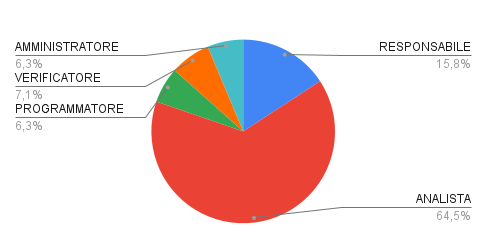
\includegraphics[width=0.6\linewidth]{grafici/6_periodo_torta.png}
  \caption{Ripartizione dei costi per ruolo nel $6^\circ$ periodo}
        \vspace{10mm}
  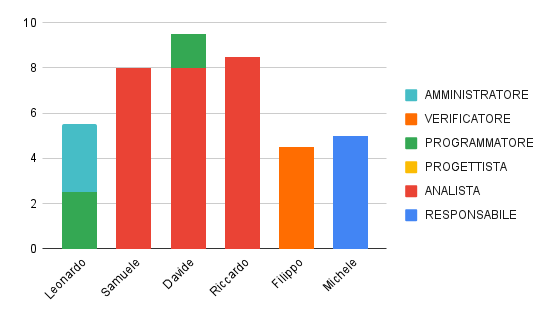
\includegraphics[width=0.7\linewidth]{grafici/6_periodo_istogramma.png}
  \caption{Ore preventivate per ciascuna persona nel $6^\circ$ periodo}
\end{figure}

\subsubsubsection{Review}
\subsubsubsubsection*{Attività svolte}
\begin{itemize}
    \item Il gruppo ritiene di aver raggiunto un livello soddisfacente per poter presentare il documento \emph{Analisi dei Requisiti} ad Imola informatica e poter dedicarsi maggiormente allo sviluppo del \emph{PoC};
    \item E' stato effettuato un incontro con il proponente il 28/2/2024 per risolvere qualche dubbio e per fare il punto della situazione. In particolare:
    \begin{itemize}
        \item Aggiornamento sullo stato dei lavori.
        \item Fissata una ipotetica data di consegna del \emph{PoC}.
        \item $\textit{Feedback}_G$ sull'attuale versione dell'\emph{Analisi dei Requisiti} e aggiornamento  sulle $\textit{tecnologie}_G$ da usare, in particolare \emph{NestJs} per il Back-End.
        \item Supporto sulla scelta della quantità di ristoranti amministrabili da un admin.
        
    \end{itemize}
\end{itemize}
\subsubsubsubsection*{Consuntivo}
\begin{table}[H]
    \centering
\begin{spreadtab}{{tabular}{|c|c|c|c|c|c|c|c|}}
    \hline
    @\textbf{Membro} & @\textbf{Re} & @\textbf{Amm} & @\textbf{An} & @\textbf{Progr} & @\textbf{Proge} & @\textbf{Ve} & @\textbf{Totale} \\
    \hline
    @ Samuele V.   & 0          & 0          & 6.42         & 0          & 0     & 0     & sum(b2:g2) \\
    @ Leonardo B.  & 0         & 3          & 0        & 1        & 0     & 0    & sum(b3:g3) \\
    @ Riccardo Z.  & 0          & 0          & 7.92          & 0          & 0     & 0   & sum(b4:g4) \\
    @ Davide B.    & 0          & 0          & 6.33       & 1.5       & 0     & 0     & sum(b5:g5) \\
    @ Michele Z.   & 4.25          & 0          & 0         & 0          & 0     & 0     & sum(b6:g6) \\
    @ Filippo T.   & 0          & 0          & 0         & 0          & 0     & 3.63     & sum(b7:g7) \\
    \hline
    @\textbf{Ore totali} & sum(b2:b7) & sum(c2:c7) & sum(d2:d7) & sum(e2:e7) & sum(f2:f7) & sum(g2:g7) &  sum(b8:g8)\\
    \hline
    @\textbf{Costo totale} & 30*b8 & 20*c8 & 25*d8 & 15*e8 & 25*f8 & 15*g8 & sum(b9:g9)\\
    \hline
\end{spreadtab}
    \caption{Consuntivo orario ed economico parziale per il sesto periodo, in base al ruolo}
    \label{tab:prev_rtb}
    \vspace{5mm}
    \textbf{Legenda:} \textit{Re} = Responsabile, \textit{Amm} = Amministratore, \textit{An} = Analista, \textit{Progr} = Programmatore, \textit{Proge} = Progettista, \textit{Ve} = Verificatore
\end{table}
\subsubsubsection{Retrospective}
Ritardata la stesura del \emph{Glossario Tecnico} a causa delle difficoltà riscontrate nel far funzionare a dovere le automazioni create per generare il documento. \\
Rallentato lo sviluppo del \emph{PoC} dato che è stata data priorità alla finalizzazione del documento \emph{Analisi dei Requisiti}.
\newpage
% Settimo periodo
\subsubsection{Settimo periodo (7/3/2024 - 24/3/2024 )}

\subsubsubsection{Planning}
%Il gruppo \emph{Ramtastic6} ha deciso di pianificare uno sprint breve della durata di una settimana per raggiungere risultati per obiettivi ben definiti e significativi seppur di durata per il loro raggiungimento contenuta.


\subsubsubsubsection*{Attività pianificate}
All'inizio del periodo ad ogni membro del gruppo sono stati assegnati ruoli specifici, di seguito riportati:
\begin{table}[H]
\centering
\begin{tabular}{|c|c|c|}
\hline
\textbf{Membro} & \textbf{Ruolo} \\
\hline
Samuele V. & Programmatore \\
\hline
Michele Z. & Programmatore \\
\hline
Leonardo B. & Amministratore \\
\hline
Riccardo Z. & Responsabile \\
\hline
Filippo T. & Programmatore \\
\hline
Davide B. & Analista \\
\hline
\end{tabular}
\caption{Ruoli assunti per ciascun membro del team all'inizio del periodo}
\end{table}

Gli obiettivi posti per lo sprint sono stati i seguenti:
\begin{itemize}
    \item Per quanto riguarda il \emph{PoC}:
    \begin{enumerate}
        \item Approfondire ulteriormente le tecnologie individuate per la sua realizzazione come Next js, Nest js e Docker e contestualmente rivedere l'organizzazione del repository per lo sviluppo.
        \item Raggiungere una configurazione accettabile per il \emph{PoC};
        \item Creare una prima versione del database (lato back-end);
        \item Raggiungere una prima implementazione della funzionalità di ricerca dei ristoranti (lato back-end e front-end);
        \item Chiedere feedback al proponente riguardo la configurazione raggiunta e consigli per quanto riguarda la feature di ordinazione.
    \end{enumerate}
    \item Aggiornare \emph{Piano di Progetto} riportando gli sprint mancanti e i nuovi sprint;
    \item Redigere una prima versione del documento \emph{Piano di Qualifica};
    \item Completare l'automazione e la stesura di una prima versione del glossario;
    \item Completare la pagina github.io riguardante il sunto dei documenti nel repository \emph{RAMtastic6.github.io}, completare l'automazione inerente e inserirla nello stesso repository;
    \item Esplorare le potenzialità di jira per analizzare il lavoro fatto.
\end{itemize}

\subsubsubsubsection*{Preventivo}
\begin{table}[H]
    \centering
\begin{spreadtab}{{tabular}{|c|c|c|c|c|c|c|c|}}
    \hline
    @\textbf{Membro} & @\textbf{Re} & @\textbf{Amm} & @\textbf{An} & @\textbf{Progr} & @\textbf{Proge} & @\textbf{Ve} & @\textbf{Totale} \\
    \hline
    @ Samuele V.   & 0          & 0          & 0        & 6.5          & 0     & 1     & sum(b2:g2) \\
    @ Leonardo B.  & 0         & 5          & 0        & 0        & 0     & 1    & sum(b3:g3) \\
    @ Riccardo Z.  & 6          & 3          & 0          & 2          & 0     & 1   & sum(b4:g4) \\
    @ Davide B.    & 0          & 1          & 2      & 0       & 0     & 4.5     & sum(b5:g5) \\
    @ Michele Z.   & 0          & 1          & 0         & 2          & 0     & 0     & sum(b6:g6) \\
    @ Filippo T.   & 0          & 0          & 0         & 5          & 0     & 0     & sum(b7:g7) \\
    \hline
    @\textbf{Ore totali} & sum(b2:b7) & sum(c2:c7) & sum(d2:d7) & sum(e2:e7) & sum(f2:f7) & sum(g2:g7) &  sum(b8:g8)\\
    \hline
    @\textbf{Costo totale} & 30*b8 & 20*c8 & 25*d8 & 15*e8 & 25*f8 & 15*g8 & sum(b9:g9)\\
    \hline
\end{spreadtab}
    \caption{Consuntivo orario ed economico parziale per il settimo periodo, in base al ruolo}
    \label{tab:prev_rtb}
    \vspace{5mm}
    \textbf{Legenda:} \textit{Re} = Responsabile, \textit{Amm} = Amministratore, \textit{An} = Analista, \textit{Progr} = Programmatore, \textit{Proge} = Progettista, \textit{Ve} = Verificatore
\end{table}
\begin{figure}[H]
  \centering
  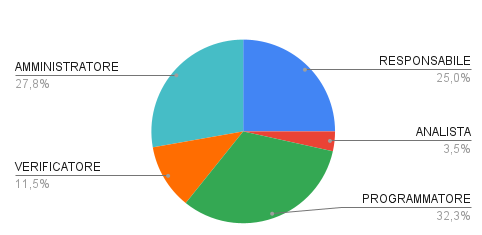
\includegraphics[width=0.6\linewidth]{grafici/7_periodo_torta.png}
  \caption{Ripartizione dei costi per ruolo nel $7^\circ$ periodo}
        \vspace{10mm}
  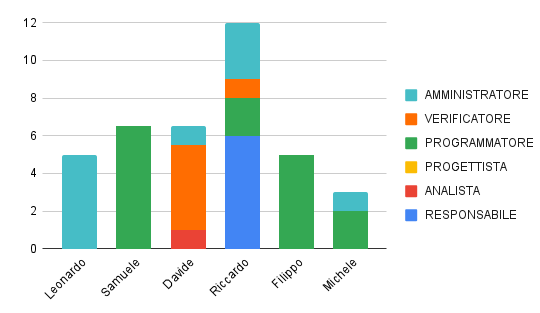
\includegraphics[width=0.7\linewidth]{grafici/7_periodo_istogramma.png}
  \caption{Ore preventivate per ciascuna persona nel $7^\circ$ periodo}
\end{figure}
\subsubsubsection{Review}
\subsubsubsubsection*{Attività svolte}
Le attività previste sono state svolte con relativo successo, in particolare:
\begin{itemize}
    \item Per quanto riguarda il \emph{PoC}:
    \begin{enumerate}
        \item I programmatori coinvolti si sono allineati sulle tecnologie;
        \item E' stata raggiunta una configurazione accettabile per il suo sviluppo;
        \item E' stata implementata una prima versione della funzionalità di ricerca dei ristoranti con la nuova configurazione (lato back-end e front-end).
    \end{enumerate}
    \item \emph{Piano di Progetto} è stato aggiornato come previsto;
    \item \emph{Piano di Qualifica} è stato iniziato come previsto;
    \item L'automazione per generare il glossario tecnico è stata completata;
    \item Una prima versione della pagina github.io; è stata completata l'automazione atta a generarla ed è stata inserita nel repository \emph{RAMtastic6.github.io};
    \item L'organizzazione del \emph{PoC} e del way of working è stata rivista come riportato nel verbale del 13/03/2024;
    \item Le potenzialità di jira sono state esplorate al fine di garantire una miglior collaborazione come riportato nel verbale del 13/03/2024;
    \item E' stato effettuato un incontro con il proponente in data 21/03/2024. In particolare:
    \begin{itemize}
        \item E' stato fornito un feedback positivo riguardante l'utilizzo dei file \emph{Json} e delle \emph{API rest} come mezzo di comunicazione tra \emph{NextJs} e \emph{NestJs}
        \item E' stato consigliato l'uso dei \emph{custom hooks};
        \item Sono stati forniti dei consigli per quanto riguarda la realizzazione della feature dell'ordinazione collaborativa. In questo contesto stato introdotto brevemente il concetto di \emph{socket};
        \item Sono stati chiariti dubbi riguardanti il ruolo del \emph{project manager}.
    \end{itemize}
\end{itemize}
\subsubsubsubsection*{Consuntivo}
\begin{table}[H]
    \centering
\begin{spreadtab}{{tabular}{|c|c|c|c|c|c|c|c|}}
    \hline
    @\textbf{Membro} & @\textbf{Re} & @\textbf{Amm} & @\textbf{An} & @\textbf{Progr} & @\textbf{Proge} & @\textbf{Ve} & @\textbf{Totale} \\
    \hline
    @ Samuele V.   & 0          & 0          & 0         & 9          & 0     & 2.5     & sum(b2:g2) \\
    @ Leonardo B.  & 0         & 5          & 2        & 0        & 0     & 1    & sum(b3:g3) \\
    @ Riccardo Z.  & 6.5          & 2.92          & 0          & 0.58          & 0     & 1.5   & sum(b4:g4) \\
    @ Davide B.    & 0          & 0.67          & 3       & 0       & 0     & 4     & sum(b5:g5) \\
    @ Michele Z.   & 0          & 3          & 0         & 3          & 0     & 0     & sum(b6:g6) \\
    @ Filippo T.   & 0          & 0          & 0         & 5.5          & 0     & 0     & sum(b7:g7) \\
    \hline
    @\textbf{Ore totali} & sum(b2:b7) & sum(c2:c7) & sum(d2:d7) & sum(e2:e7) & sum(f2:f7) & sum(g2:g7) &  sum(b8:g8)\\
    \hline
    @\textbf{Costo totale} & 30*b8 & 20*c8 & 25*d8 & 15*e8 & 25*f8 & 15*g8 & sum(b9:g9)\\
    \hline
\end{spreadtab}
    \caption{Consuntivo orario ed economico parziale per il settimo periodo, in base al ruolo}
    \label{tab:prev_rtb}
    \vspace{5mm}
    \textbf{Legenda:} \textit{Re} = Responsabile, \textit{Amm} = Amministratore, \textit{An} = Analista, \textit{Progr} = Programmatore, \textit{Proge} = Progettista, \textit{Ve} = Verificatore
\end{table}
\subsubsubsection{Retrospective}
Il rischio atteso è stato principalmente: \nameref{rt:1}, in quanto per la prima volta i componenti del gruppo si sono interfacciati con il framework \emph{NestJs}. Tuttavia, i programmatori dopo diverse ore di studio individuale hanno dimostrato di aver compreso le tecnologie studiate raggiungendo una configurazione stabile per lo sviluppo del \emph{PoC}.
\newline Tra i rischi attesi verificati rientra la scarsa attenzione avuta in precedenza riguardo il conteggio delle ore e la difficoltà da parte del responsabile nel calcolo delle ore prima dell'introduzione dello strumento \emph{Jira}. Per mitigare questo rischi si è deciso per il periodo successivo di introdurre un secondo responsabile e di organizzare tramite file \emph{Excel} le ore in modo sistematico e preciso.
\newline
In questa fase i costi emersi dal consuntivo hanno ecceduto quelli del preventivo facendo verificare il rischio di valutazione erronea delle ore assegnate; in particolare si rileva un eccesso nei ruoli di \emph{Amministratore} e di \emph{Programmatore} in quanto:
\begin{itemize}
    \item Per l'amministratore sono emerse problematiche riguardanti il funzionamento dell'automazione del glossario e un cambio in corsa per quanto riguarda l'automazione del sunto dei documenti;
    \item Per il ruolo di programmatore essendo tecnologie nuove per i componenti del gruppo si è sottostimata la loro applicazione e coesione nell'ambito di un progetto complesso.
\end{itemize}


\newpage
% Ottavo periodo
\subsubsection{Ottavo periodo (25/3/2024 - 7/4/2024 )}
\subsubsubsection{Planning}
\subsubsubsubsection*{Attività pianificate}
All'inizio del periodo ad ogni membro del gruppo sono stati assegnati ruoli specifici, di seguito riportati:
\begin{table}[H]
\centering
\begin{tabular}{|c|c|c|}
\hline
\textbf{Membro} & \textbf{Ruolo} \\
\hline
Samuele V. & Programmatore \\
\hline
Michele Z. & Amministratore \\
\hline
Leonardo B. & Programmatore \\
\hline
Riccardo Z. & Responsabile \\
\hline
Filippo T. & Programmatore \\
\hline
Davide B. & Responsabile \\
\hline
\end{tabular}
\caption{Ruoli assunti per ciascun membro del team all'inizio del periodo}
\end{table}
Gli obiettivi posti per lo sprint sono stati i seguenti:
\begin{itemize}
    \item Per quanto riguarda il \emph{PoC}:
    \begin{itemize}
        \item Raggiungere una prima implementazione della schermata di login (lato front-end);
        \item Raggiungere una prima implementazione della funzionalità di prenotazione (lato back-end e front-end);
        \item Raggiungere una prima implementazione della funzionalità di ordinazione (lato back-end e front-end) esplorando i \emph{socket} per la comunicazione bidirezionale.
    \end{itemize}
    \item Aggiornare il documento \emph{Norme di Progetto} apportando le seguenti modifiche:
    \begin{itemize}
        \item Specificare in modo maggiormente dettagliato i ruoli;
        \item Aggiungere le nuove repository create e la loro organizzazione;
        \item Aggiungere tra i processi di supporto le attività di verifica e di gestione della qualità;
        \item Specificare l'utilizzo delle nuove automazioni aggiunte recentemente.
    \end{itemize}
    \item Redigere una prima versione del glossario;
    \item Redigere una prima versione della sezione \emph{Qualità di Prodotto} e di \emph{Test di Sistema} nel documento \emph{Piano di Qualifica};
    \item Aggiornare i periodi precedenti nel \emph{Piano di Progetto} andando a definire un modo sistematico per calcolare le ore preventivate ed effettive;
    \item Rivedere i costi e le scadenze in fase di candidatura.
\end{itemize}
\subsubsubsubsection*{Preventivo}
\begin{table}[H]
    \centering
\begin{spreadtab}{{tabular}{|c|c|c|c|c|c|c|c|}}
    \hline
    @\textbf{Membro} & @\textbf{Re} & @\textbf{Amm} & @\textbf{An} & @\textbf{Progr} & @\textbf{Proge} & @\textbf{Ve} & @\textbf{Totale} \\
    \hline
    @ Samuele V.   & 0          & 0          & 0        & 5          & 0     & 0     & sum(b2:g2) \\
    @ Leonardo B.  & 0         & 0          & 0        & 5        & 0     & 0    & sum(b3:g3) \\
    @ Riccardo Z.  & 4.5          & 0          & 0          & 0.17          & 0     & 1.5  & sum(b4:g4) \\
    @ Davide B.    & 4          & 0         & 0      & 0       & 0     & 0     & sum(b5:g5) \\
    @ Michele Z.   & 0          & 4          & 0         & 0          & 0     & 0.17     & sum(b6:g6) \\
    @ Filippo T.   & 0          & 0          & 0         & 5          & 0     & 0     & sum(b7:g7) \\
    \hline
    @\textbf{Ore totali} & sum(b2:b7) & sum(c2:c7) & sum(d2:d7) & sum(e2:e7) & sum(f2:f7) & sum(g2:g7) &  sum(b8:g8)\\
    \hline
    @\textbf{Costo totale} & 30*b8 & 20*c8 & 25*d8 & 15*e8 & 25*f8 & 15*g8 & sum(b9:g9)\\
    \hline
\end{spreadtab}
    \caption{Preventivo orario ed economico parziale per l'ottavo periodo, in base al ruolo}
    \label{tab:prev_rtb}
    \vspace{5mm}
    \textbf{Legenda:} \textit{Re} = Responsabile, \textit{Amm} = Amministratore, \textit{An} = Analista, \textit{Progr} = Programmatore, \textit{Proge} = Progettista, \textit{Ve} = Verificatore
\end{table}

\begin{figure}[H]
  \centering
  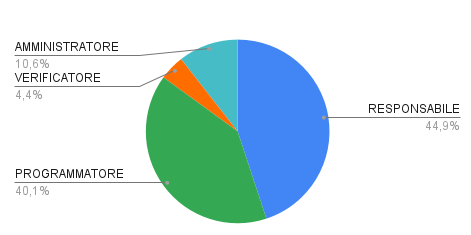
\includegraphics[width=0.6\linewidth]{grafici/8_periodo_torta.png}
  \caption{Ripartizione dei costi per ruolo nel $8^\circ$ periodo}
        \vspace{5mm}
  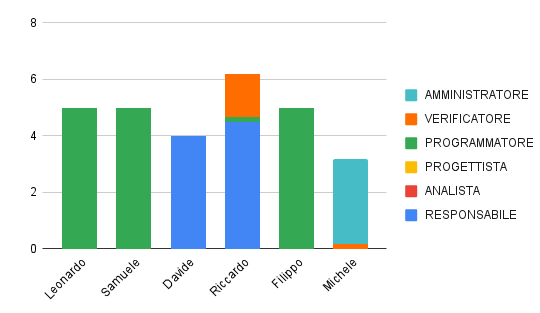
\includegraphics[width=0.7\linewidth]{grafici/8_periodo_istogramma.png}
  \caption{Ore preventivate per ciascuna persona nel $8^\circ$ periodo}
\end{figure}

\subsubsubsection{Review}
\subsubsubsubsection*{Attività svolte}
Le attività svolte in questo periodo sono state le seguenti:
\begin{itemize}
    \item Redatta ed approvata una prima versione del glossario tecnico;
    \item Redatte le sezioni \emph{Qualità di Prodotto} e \emph{Test di sistema} nel documento \emph{Piano di Qualifica};
    \item Aggiornato \emph{Norme di Progetto} con le attività di verifica, gestione della qualità e la procedura per la redazione del glossario;
    \item Rivisti i costi stabiliti in fase di candidatura;
    \item Integrati i websocket nel PoC, implementate le funzionalità di prenotazione e ordinazione, non quella di login e raggiunta una configurazione soddisfacente;
    \item Richiesto un incontro con il prof. Cardin per la prima parte della revisione RTB;
    \item Richiesto e fissato un incontro con il proponente in data 11 aprile per presentare il PoC.
\end{itemize}
\subsubsubsubsection*{Consuntivo}
\begin{table}[H]
    \centering
\begin{spreadtab}{{tabular}{|c|c|c|c|c|c|c|c|}}
    \hline
    @\textbf{Membro} & @\textbf{Re} & @\textbf{Amm} & @\textbf{An} & @\textbf{Progr} & @\textbf{Proge} & @\textbf{Ve} & @\textbf{Totale} \\
    \hline
    @ Samuele V.   & 0          & 0          & 0         & 6          & 0     & 0     & sum(b2:g2) \\
    @ Leonardo B.  & 0         & 0          & 0        & 5.42        & 0     & 0    & sum(b3:g3) \\
    @ Riccardo Z.  & 6.75          & 0          & 0          & 0.17         & 0     & 2   & sum(b4:g4) \\
    @ Davide B.    & 5          & 0         & 0       & 0       & 0     & 0     & sum(b5:g5) \\
    @ Michele Z.   & 0          & 4.25          & 0         & 0          & 0     & 0.17     & sum(b6:g6) \\
    @ Filippo T.   & 0          & 0          & 0         & 8.5          & 0     & 0     & sum(b7:g7) \\
    \hline
    @\textbf{Ore totali} & sum(b2:b7) & sum(c2:c7) & sum(d2:d7) & sum(e2:e7) & sum(f2:f7) & sum(g2:g7) &  sum(b8:g8)\\
    \hline
    @\textbf{Costo totale} & 30*b8 & 20*c8 & 25*d8 & 15*e8 & 25*f8 & 15*g8 & sum(b9:g9)\\
    \hline
\end{spreadtab}
    \caption{Consuntivo orario ed economico parziale per l'ottavo periodo, in base al ruolo}
    \label{tab:prev_rtb}
    \vspace{5mm}
    \textbf{Legenda:} \textit{Re} = Responsabile, \textit{Amm} = Amministratore, \textit{An} = Analista, \textit{Progr} = Programmatore, \textit{Proge} = Progettista, \textit{Ve} = Verificatore
\end{table}
\subsubsubsection{Retrospective}
Dal presente periodo sono emersi i seguenti elementi:
\begin{itemize}
    \item E' stato riscontrato durante un meeting un errore sull'automazione per i riferimenti del glossario, si è dunque deciso di intervenire assegnando la task apposita ad uno dei membri del gruppo dunque ricorrendo ad un innalzamento dei costi. Per mitigare tale problema si è dovuta stabilire una procedura di inserimento delle parole del glossario nei documenti e verifica dei documenti da inserire nei prossimi periodi.
    \item La finalizzazione del documento \emph{Analisi dei Requisiti} si è rivelata più difficoltosa del previsto, portando ad un innalzamento dei costi e facendo emergere delle attività di verifica lacunose e da rivedere per le prossime stesure dei documenti. Per mitigare tale problema si è stabilito che debbano esistere delle procedure da seguire per poter segnare come "verificato" un documento, in particolare si aggiorneranno nei prossimi periodi le sezioni relative a ciascun documento.
\end{itemize}


%\subsubsubsubsection*{Rischi verificati}
%\subsubsubsubsection*{Analisi retrospettiva}
\newpage
% Nono periodo
\subsubsection{Nono periodo (8/4/2024 - 27/4/2024)}
\subsubsubsection{Planning}
\subsubsubsubsection*{Attività pianificate}
Gli obiettivi posti per lo sprint sono stati i seguenti:
\begin{itemize}
    \item Effettuare un incontro con il proponente fissato in data 10 Aprile in cui mostrare quanto fatto nel PoC;
    \item Effettuare il colloquio con il prof. Cardin per la revisione RTB in data 12 Aprile per il quale si vuole:
    \begin{itemize}
        \item Preparare le diapositive per il colloquio;
        \item Preparare la lettera di presentazione per la fase RTB.
    \end{itemize}
    \item Per quanto riguarda il Piano di Qualifica si vuole:
    \begin{itemize}
        \item Individuare le metriche da inserire nella sezione \emph{"Cruscotto di valutazione della qualità"};
        \item Stilare di conseguenza la sezione di \emph{"Modifiche migliorative"};
        \item Aggiornare la sezione \emph{Test di sistema} in base a quanto riportato nell'ultimo aggiornamento dell'Analisi dei Requisiti in particolare riguardo ai requisiti.
    \end{itemize}
    \item Effettuare delle correzioni (eventuali) all'Analisi dei Requisiti fornite dal prof. Cardin in fase di revisione RTB.
    \item Aggiornare Norme di Progetto, inserendo alcune sezioni mancanti come \emph{Validazione}, \emph{repository Proof of Concept} e inserendo come vengono gestite le procedure per alcuni ruoli.
\end{itemize}
\subsubsubsubsection*{Preventivo}
\begin{table}[H]
    \centering
\begin{spreadtab}{{tabular}{|c|c|c|c|c|c|c|c|}}
    \hline
    @\textbf{Membro} & @\textbf{Re} & @\textbf{Amm} & @\textbf{An} & @\textbf{Progr} & @\textbf{Proge} & @\textbf{Ve} & @\textbf{Totale} \\
    \hline
    @ Samuele V.   & 0          & 2.42          & 0         & 0.25          & 0     & 0.55     & sum(b2:g2) \\
    @ Leonardo B.  & 0         & 0          & 1        & 0        & 0     & 2.92    & sum(b3:g3) \\
    @ Riccardo Z.  & 1.5          & 2.5          & 0          & 0.67         & 0     & 0.25  & sum(b4:g4) \\
    @ Davide B.    & 2.5          & 2.5         & 0       & 0       & 0     & 0     & sum(b5:g5) \\
    @ Michele Z.   & 0          & 2.5          & 1.5         & 0          & 0     & 1.67     & sum(b6:g6) \\
    @ Filippo T.   & 0          & 1.83          & 2         & 0.33          & 0     & 0     & sum(b7:g7) \\
    \hline
    @\textbf{Ore totali} & sum(b2:b7) & sum(c2:c7) & sum(d2:d7) & sum(e2:e7) & sum(f2:f7) & sum(g2:g7) &  sum(b8:g8)\\
    \hline
    @\textbf{Costo totale} & 30*b8 & 20*c8 & 25*d8 & 15*e8 & 25*f8 & 15*g8 & sum(b9:g9)\\
    \hline
\end{spreadtab}
    \caption{Preventivo orario ed economico parziale per il nono periodo, in base al ruolo}
    \label{tab:prev_rtb}
    \vspace{5mm}
    \textbf{Legenda:} \textit{Re} = Responsabile, \textit{Amm} = Amministratore, \textit{An} = Analista, \textit{Progr} = Programmatore, \textit{Proge} = Progettista, \textit{Ve} = Verificatore
\end{table}
\subsubsubsection{Review}
\subsubsubsubsection*{Attività svolte}
Le attività svolte in questo periodo sono state le seguenti:
\begin{itemize}
    \item Effettuato un incontro con il proponente per mostrare quanto sviluppato per il PoC in cui:
    \begin{itemize}
        \item è emerso l'apprezzamento per la feature di ordinazione collaborativa;
        \item è emerso che in futuro si debba prendere in considerazione la paginazione per gestire una grande mole di dati in funzionalità quali la ricerca del ristorante;
        \item si è discusso di architetture come Kafka;
        \item si è parlato della possibilità di impostare un progetto implementando un'architettura a microservizi.
    \end{itemize}
    \item Effettuato il colloquio con il prof. Cardin per la revisione RTB presentando le relative diapositive, il quale è risultato in un semaforo verde con le relative correzioni da effettuare al documento di Analisi dei Requisiti.
    \item Aggiornato Norme di Progetto e inserite le sezioni mancanti;
    \item Aggiornato Piano di Qualifica e inserite le metriche nella sezione riguardante il cruscotto;
    \item Corretto il documento di Analisi dei Requisiti con le indicazioni del prof. Cardin;
    \item Aggiornato il presente documento con i relativi grafici per ogni periodo;
    \item Preparata la lettera di presentazione e decisa la data di consegna del progetto rivista.
\end{itemize}
\subsubsubsubsection*{Consuntivo}
\begin{table}[H]
    \centering
\begin{spreadtab}{{tabular}{|c|c|c|c|c|c|c|c|}}
    \hline
    @\textbf{Membro} & @\textbf{Re} & @\textbf{Amm} & @\textbf{An} & @\textbf{Progr} & @\textbf{Proge} & @\textbf{Ve} & @\textbf{Totale} \\
    \hline
    @ Samuele V.   & 0          & 2.08          & 0         & 0.17          & 0     & 0.58     & sum(b2:g2) \\
    @ Leonardo B.  & 0         & 0          & 1        & 0        & 0     & 2.67    & sum(b3:g3) \\
    @ Riccardo Z.  & 1.17          & 1.5          & 0          & 0.67         & 0     & 0.42   & sum(b4:g4) \\
    @ Davide B.    & 2          & 2         & 0       & 0       & 0     & 0     & sum(b5:g5) \\
    @ Michele Z.   & 0          & 1.5          & 0         & 0          & 0     & 0.83     & sum(b6:g6) \\
    @ Filippo T.   & 0          & 1.33          & 1.75         & 0.33          & 0     & 0     & sum(b7:g7) \\
    \hline
    @\textbf{Ore totali} & sum(b2:b7) & sum(c2:c7) & sum(d2:d7) & sum(e2:e7) & sum(f2:f7) & sum(g2:g7) &  sum(b8:g8)\\
    \hline
    @\textbf{Costo totale} & 30*b8 & 20*c8 & 25*d8 & 15*e8 & 25*f8 & 15*g8 & sum(b9:g9)\\
    \hline
\end{spreadtab}
    \caption{Consuntivo orario ed economico parziale per il nono periodo, in base al ruolo}
    \label{tab:prev_rtb}
    \vspace{5mm}
    \textbf{Legenda:} \textit{Re} = Responsabile, \textit{Amm} = Amministratore, \textit{An} = Analista, \textit{Progr} = Programmatore, \textit{Proge} = Progettista, \textit{Ve} = Verificatore
\end{table}

\begin{figure}[H]
  \centering
  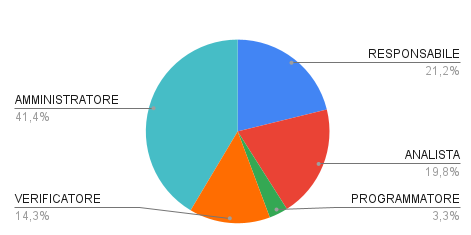
\includegraphics[width=0.6\linewidth]{grafici/9_periodo_torta.png}
  \caption{Ripartizione dei costi per ruolo nel $9^\circ$ periodo}
        \vspace{5mm}
  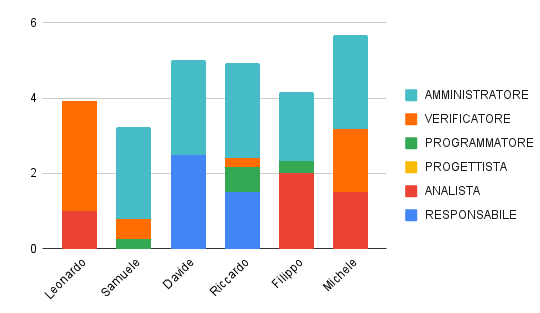
\includegraphics[width=0.7\linewidth]{grafici/9_periodo_istogramma.png}
  \caption{Ore preventivate per ciascuna persona nel $9^\circ$ periodo}
\end{figure}

\subsubsubsection{Retrospective}
La stesura dei documenti si è rilevata più' dispendiosa del previsto e tali documenti sono stati approvati più' tardi rispetto a quanto stabilito all'inizio del periodo. In particolare:
\begin{itemize}
    \item Per l'Analisi dei Requisiti non era chiaro ad alcuni membri del gruppo come poter effettuare le correzioni indicate;
    \item E' emerso che in futuro si dovranno distribuire più' correttamente le attività in base alle disponibilità di ciascun membro.
\end{itemize}
\newpage

\subsection{Verso la PB}
Successivamente all'analisi dei costi intrapresi durante la $\textit{RTB}_G$ e le criticità emerse, viene indicata come data di consegna del progetto il giorno 2024/07/05 e nel mentre viene confermato il budget previsto all'inizio del progetto, ovvero 11520 \euro. Viene inoltre elaborato un $\textit{preventivo}_G$ per questa fase riportato nella sezione 5.\\
La revisione $\textit{PB}_G$ (\emph{Product baseline}) comprende diversi obiettivi da soddisfare, di seguito elencati:
\begin{itemize}
    \item valutare la baseline architetturale del prodotto $\textit{software}_G$ tramite il documento \textbf{Specifica Tecnica};
    \item realizzare un prodotto dimostrabile tramite l'\textbf{MVP} (\emph{Minimum Viable Product}).
\end{itemize}
A supporto di tali attività vi è la $\textit{manutenzione}_G$ della documentazione citata nella sezione riguardante la revisione $\textit{RTB}_G$:
\begin{itemize}
    \item il presente \textbf{Piano di Progetto};
    \item il \textbf{Piano di Qualifica};
    \item il \textbf{Glossario};
    \item \textbf{Norme di Progetto};
    \item \textbf{Analisi dei Requisiti};
    \item \textbf{Verbali} interni ed esterni.
\end{itemize}
In supporto a tali attività viene fornito anche:
\begin{itemize}
    \item il \textbf{Manuale Utente}:\\
    documento che illustra le funzionalità del prodotto e fornisce una guida all'uso destinata agli utenti finali.
\end{itemize}
Analogamente a come fatto per la revisione $\textit{RTB}_G$, ciascuno dei documenti elencati dovrà essere archiviato in un $\textit{repository}_G$ accessibile dal committente e dal proponente e ciascuno degli obiettivi sopra elencati ed evidenziati in grassetto corrisponderà nel $\textit{software}_G$ di $\textit{versionamento}_G$ $\textit{jira}_G$ ad un elemento di tipo \emph{"Epic"} utilizzato per raggruppare un insieme di task di minori dimensioni.\\
I periodi presentati in questa sezione saranno descritti tramite le fasi di \emph{sprint planning}, \emph{sprint review} e \emph{sprint retrospective}. Viene ricordato che in ogni periodo, le ore che riguardano il $\textit{preventivo}_G$ e il $\textit{consuntivo}_G$ sono riportate in formato decimale in quanto rappresentano in modo più dettagliato le task assegnate.

\begin{comment}

\begin{table}[h]
\centering
\captionsetup{justification=centering}
\begin{tabular}{|c|c|c|}
\hline
\textbf{Data di inizio} & \textbf{Data di fine prevista} & \textbf{Data di superamento della revisione PB} \\
\hline
2024/05/03 & 2024/07/05 & N/A \\
\hline
\end{tabular}
\caption{Periodo verso la revisione PB}
\end{table}

\end{comment}

\newpage
% Decimo periodo
\subsubsection{Decimo periodo (2024/05/03 - 2024/05/19)}
\subsubsubsection{Planning}
In questa prima fase, in vista della revisione $\textit{PB}_G$, si è cercato di definire le prime attività, le quali riguardano principalmente la consegna di un $\textit{MVP}_G$. Di conseguenza, molte risorse sono state destinate ai ruoli dei Progettisti e dei Programmatori. \\
A causa dei ritardi considerevoli avuti dal gruppo, si è convenuto, come da suggerimento del prof. Vardanega durante l'ultima parte di revisione $\textit{RTB}_G$, di suddividere, nel corso di una settimana, il gruppo tramite due formazioni composte da tre membri, studiando separatamente le fasi relative alla progettazione e al testing, condividendo a fine della settimana (il 2024/05/10) le informazioni apprese. \\
La seconda parte del periodo, invece, si è concentrata sullo sviluppo dei requisiti necessari per l'$\textit{MVP}_G$ e della messa in pratica del materiale appreso in precedenza, redigendo, parallelamente, il documento di Specifica Tecnica.
\subsubsubsubsection*{Attività pianificate}
Gli obiettivi posti per lo $\textit{sprint}_G$ sono stati i seguenti:
\begin{itemize}
    \item Effettuare degli incontri con il proponente per discutere dei requisti per l'$\textit{MVP}_G$ e dei consigli sull'$\textit{architettura}_G$ da adottare;
    \item Aggiornare il documento di Analisi dei Requisiti;
    \item Aggiornare i documenti, il $\textit{repository}_G$ e il sito web in base alle indicazione fornite in sede di revisione $\textit{RTB}_G$ dal prof. Vardanega:
    \begin{itemize}
        \item Cambiare impostazione dei verbali;
        \item Cambiare impostazione del sito web;
        \item Cambiare impostazione del $\textit{repository}_G$ riservato alla documentazione;
        \item Cambiare impostazione del glossario tecnico;
        \item Modificare $\textit{Norme di Progetto}_G$;
        \item Modificare $\textit{Piano di Qualifica}_G$;
        \item Modificare il presente $\textit{Piano di Progetto}_G$.
    \end{itemize}
    \item Iniziare la stesura del documento di Specifica Tecnica;
    \item Studiare separatamente, tramite una formazione di gruppi composti da tre membri, le fasi relative alla progettazione e al testing, condividendo a fine della settimana (il 2024/05/10) le informazioni apprese. 
    \item Configurare il $\textit{repository}_G$ dedicato all'$\textit{MVP}_G$, inserendo automazioni per effettuare il testing del codice.
    \item Sviluppare alcuni requisiti obbligatori per l'$\textit{MVP}_G$.
\end{itemize}
\subsubsubsubsection*{Preventivo}
\begin{table}[H]
    \centering
\begin{spreadtab}{{tabular}{|c|c|c|c|c|c|c|c|}}
    \hline
    @\textbf{Membro} & @\textbf{Re} & @\textbf{Amm} & @\textbf{An} & @\textbf{Progr} & @\textbf{Proge} & @\textbf{Ve} & @\textbf{Totale} \\
    \hline
    @ Samuele V.   & 2          & 2.67          & 0         & 12.01          & 2.5     & 3.92     & sum(b2:g2) \\
    @ Leonardo B.  & 0         & 1.92          & 0.67        & 0.5        & 0     & 2.17    & sum(b3:g3) \\
    @ Riccardo Z.  & 4.33          & 2.17          & 0          & 5.59         & 4.17     & 1.5 & sum(b4:g4) \\
    @ Davide B.    & 0          & 1.25         & 0.33       & 0       & 0     & 0.17     & sum(b5:g5) \\
    @ Michele Z.   & 0          & 0          & 0         & 0          & 0     & 0.5     & sum(b6:g6) \\
    @ Filippo T.   & 0          & 0          & 0         & 1.33          & 0     & 0.17      & sum(b7:g7) \\
    \hline
    @\textbf{Ore totali} & sum(b2:b7) & sum(c2:c7) & sum(d2:d7) & sum(e2:e7) & sum(f2:f7) & sum(g2:g7) &  sum(b8:g8)\\
    \hline
    @\textbf{Costo totale} & 30*b8 & 20*c8 & 25*d8 & 15*e8 & 25*f8 & 15*g8 & sum(b9:g9)\\
    \hline
\end{spreadtab}
    \caption{Preventivo orario ed economico parziale per il decimo periodo, in base al ruolo}
    \label{tab:prev_rtb}
    \vspace{5mm}
    \textbf{Legenda:} \textit{Re} = Responsabile, \textit{Amm} = Amministratore, \textit{An} = Analista, \textit{Progr} = Programmatore, \textit{Proge} = Progettista, \textit{Ve} = Verificatore
\end{table}
\begin{figure}[H]
    \centering
  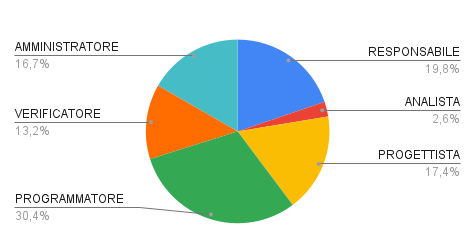
\includegraphics[width=0.6\linewidth]{grafici/10_periodo_torta.png}
  \caption{Preventivo ripartizione dei costi per ruolo nel $10^\circ$ periodo}
        \vspace{5mm}
  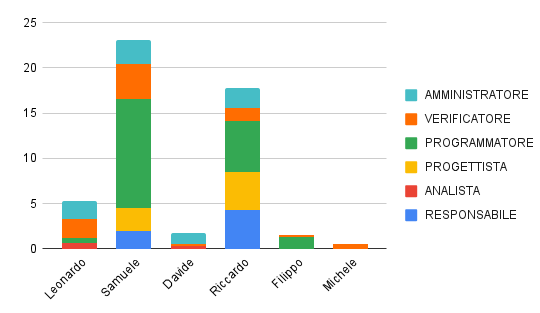
\includegraphics[width=0.7\linewidth]{grafici/10_periodo_istogramma.png}
  \caption{Ore preventivate per ciascuna persona nel $10^\circ$ periodo}
\end{figure}
\subsubsubsection{Review}
Le attività preventivate sono state svolte con successo, risultando un rallentamento solamente per quanto riguarda l'aggiornamento dei documenti secondo le indicazioni fornite in sede di revisione $\textit{RTB}_G$.
\subsubsubsubsection*{Attività svolte}
Le attività svolte in questo periodo sono state le seguenti:
\begin{itemize}
    \item Effettuati tre incontri con il proponente per discutere dei requisiti e dubbi riguardanti la progettazione e la $\textit{codifica}_G$;
\item Aggiornato il documento Analisi dei Requisiti in base a quanto riportato dal proponente relativo all'interazione con lo staff del ristorante tramite chat;
\item Aggiornato il documento $\textit{Norme di Progetto}_G$ con le procedure per la $\textit{codifica}_G$ e la verifica del codice;
\item Aggiornato il documento $\textit{Piano di Qualifica}_G$ con alcune metriche riguardanti la fase di testing;
\item A seguito della valutazione $\textit{RTB}_G$:
\begin{itemize}
    \item Cambiata l'impostazione dei verbali;
    \item Cambiata l'impostazione del sito web;
    \item Cambiata l'impostazione del $\textit{repository}_G$ riservato alla documentazione;
    \item Cambiata l'impostazione del glossario tecnico.
\end{itemize}
\item Completata la progettazione logica e ricevuto $\textit{feedback}_G$ positivo da parte del proponente;
\item Effettuata una prima stesura del documento di Specifica Tecnica;
\item Sviluppati alcuni requisiti funzionali;
\item Implementati i primi $\textit{test}_G$ di unità;
\item Progettato il $\textit{sistema}_G$ di notifica dal punto di vista logico e ricevuto un riscontro positivo da parte del proponente.
\end{itemize}
\subsubsubsubsection*{Consuntivo}
\begin{table}[H]
    \centering
\begin{spreadtab}{{tabular}{|c|c|c|c|c|c|c|c|}}
    \hline
    @\textbf{Membro} & @\textbf{Re} & @\textbf{Amm} & @\textbf{An} & @\textbf{Progr} & @\textbf{Proge} & @\textbf{Ve} & @\textbf{Totale} \\
    \hline
    @ Samuele V.   & 2          & 2.67          & 0        & 15.26        & 2.5     & 3.92    & sum(b2:g2) \\
    @ Leonardo B.  & 0         & 2.17          & 0.67        & 0.5        & 0     & 3.25    & sum(b3:g3) \\
    @ Riccardo Z.  & 4.33         & 1.72          & 0          & 6.75         & 4.17     & 1.92   & sum(b4:g4) \\
    @ Davide B.    & 0          & 1         & 1.5       & 0       & 0     & 1     & sum(b5:g5) \\
    @ Michele Z.   & 0          & 0          & 0         & 1.83          & 0     & 0.17     & sum(b6:g6) \\
    @ Filippo T.   & 0          & 0          & 0         & 0          & 0     & 1     & sum(b7:g7) \\
    \hline
    @\textbf{Ore totali} & sum(b2:b7) & sum(c2:c7) & sum(d2:d7) & sum(e2:e7) & sum(f2:f7) & sum(g2:g7) &  sum(b8:g8)\\
    \hline
    @\textbf{Costo totale} & 30*b8 & 20*c8 & 25*d8 & 15*e8 & 25*f8 & 15*g8 & sum(b9:g9)\\
    \hline
\end{spreadtab}
    \caption{Consuntivo orario ed economico parziale per il decimo periodo, in base al ruolo}
    \label{tab:prev_rtb}
    \vspace{5mm}
    \textbf{Legenda:} \textit{Re} = Responsabile, \textit{Amm} = Amministratore, \textit{An} = Analista, \textit{Progr} = Programmatore, \textit{Proge} = Progettista, \textit{Ve} = Verificatore
\end{table}

\begin{comment}
\begin{figure}[H]
  \centering
  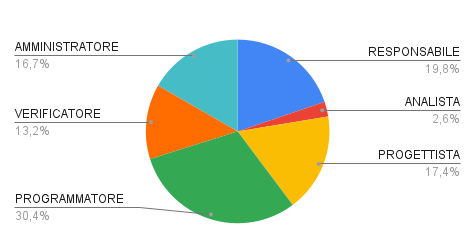
\includegraphics[width=0.6\linewidth]{grafici/10_periodo_torta.png}
  \caption{Ripartizione dei costi per ruolo nel $10^\circ$ periodo}
        \vspace{5mm}
  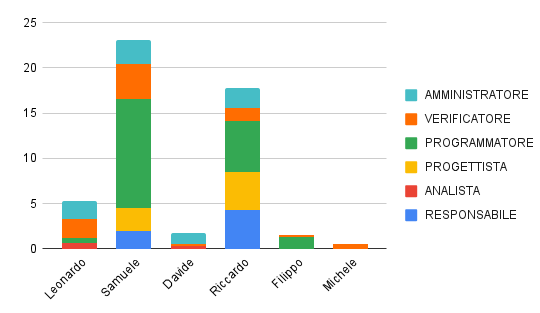
\includegraphics[width=0.7\linewidth]{grafici/10_periodo_istogramma.png}
  \caption{Ore preventivate per ciascuna persona nel $10^\circ$ periodo}
\end{figure}
\end{comment}

\begin{figure}[H]
  \centering
  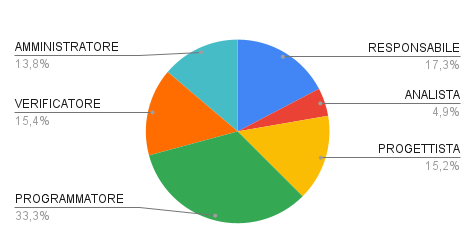
\includegraphics[width=0.6\linewidth]{grafici/10_periodo_torta_consuntivo.png}
  \caption{Consuntivo ripartizione dei costi per ruolo nel $10^\circ$ periodo}
  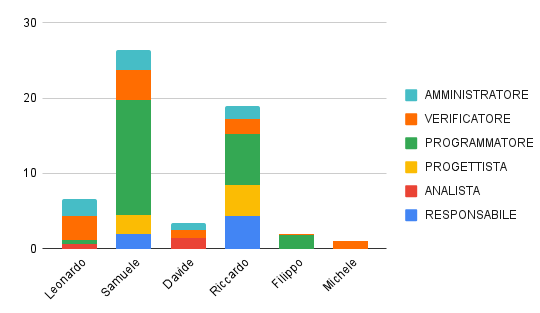
\includegraphics[width=0.7\linewidth]{grafici/10_periodo_instogramma_consuntivo.png}
  \caption{Ore svolte per ciascuna persona nel $10^\circ$ periodo}
\end{figure}

\subsubsubsection{Retrospective}
\paragraph*{Gestione dei Rischi}
I $\textit{rischi}_G$ occorsi per tale periodo sono stati i seguenti:
\begin{itemize}
    \item \nameref{ro:1}: la scarsa esperienza nell'organizzazione di un progetto complesso ha causato un rallentamento previsto nel corso dello $\textit{sprint}_G$. In particolare si è rilevata una sottostima nelle attività di verifica e di programmazione.
    \begin{itemize}
        \item \textbf{Esito mitigazione}: il continuo colloquio tra il responsabile e i membri del gruppo hanno fatto sì di poter estendere la durata delle attività segnalate in modo ragionevole.
        \item \textbf{Impatto}: sono state spese risorse significative non previste andando ad impattare sul modo di calcolare le ore per il progettista e per il verificatore per quanto riguarda la $\textit{codifica}_G$.
    \end{itemize}
    \item \nameref{ro:3}: un membro del gruppo, a causa di impegni lavorativi, non ha potuto eseguire le task assegnatoli.
    \begin{itemize}
        \item \textbf{Esito mitigazione}: le task assegnate al membro del gruppo sono state scelte tra le meno urgenti e "bloccanti" rispetto al resto del progetto non causando rallentamenti significativi.
        \item \textbf{Impatto}: la poca partecipazione nelle attività principali potrebbe causare un rallentamento ulteriore nello studio delle $\textit{tecnologie}_G$ e della progettazione. Al momento non si registrano conseguenze considerevoli. 
    \end{itemize}
    \item \nameref{ro:4}: la scarsa chiarezza nella gestione dei ruoli e delle attività ha causato un rallentamento previsto nel corso dello $\textit{sprint}_G$.
    \begin{itemize}
        \item \textbf{Esito mitigazione}: le attività di studio individuale e di gruppo avevano lo scopo di apprendere come maggiore efficienza i compiti di progettazione e di testing oltre che di chiarire maggiormente i ruoli del progettista e dell'amministratore, tuttavia tutto ciò è risultato per alcuni membri del gruppo in poca chiarezza per quanto riguarda le attività individuali e per la gestione dei ruoli. 
        \item \textbf{Impatto}: alcuni membri del gruppo avevano compreso poco il ruolo assegnatoli rispetto ad altri. Il fatto che alcuni membri del gruppo fossero "più' attivi" ha causato un eccessivo rilassamento in merito allo studio individuale che è andato ad impattare sulla stesura del documento di Specifica Tecnica e lo sviluppo dei $\textit{test}_G$ di unità oltre che sulle attività inerenti future.
    \end{itemize}
    \item \nameref{ro:5}: la scarsa esperienza nella progettazione e nel testing ha causato un rallentamento previsto nel corso dello $\textit{sprint}_G$.
    \begin{itemize}
        \item \textbf{Esito mitigazione}: le attività di studio individuale e il confronto di gruppo e gli incontri frequenti con il proponente sono stati gli elementi principali per mitigare tale rischio. In particolare per ogni risultato ottenuto in fase di testing e di progettazione, si è data una dimostrazione al proponente, ottenendone un riscontro tempestivo. I risultati sono stati soddisfacenti e in linea con quanto preventivato.
        \item \textbf{Impatto}: dopo un primo periodo di incertezza, i membri del gruppo hanno dimostrato di aver appreso maggiormente nell'ambito del testing, meno nell'ambito della progettazione. Nonostante questo, non si sono registrate conseguenze significative.
    \end{itemize}
\end{itemize}
\paragraph*{Considerazioni e pianificazione futura}
\begin{itemize}
    \item Sebbene la progettazione logica sia stata compresa, come dimostra il $\textit{feedback}_G$ positivo da parte del proponente, quella di $\textit{sistema}_G$ presenta alcune parti incomprese relative alle definizione dei $\textit{design}_G$ pattern architetturali e la formazione dei primi diagrammi $\textit{UML}_G$. In futuro, tramite un incontro con il prof. Cardin, si dovrà intervenire su questi dubbi.
    \item Alcuni membri del gruppo, spinti da esigenze personali, sono risultati maggiormente motivati a svolgere le attività assegnateli rispetto ad altri. In particolare, si registra uno sbilanciamento delle ore considerevole tra alcuni di essi. Inoltre, il monte ore raggiunto fino a questo momento non permette di far arrivare alla conclusione tutti i membri del gruppo in un tempo ragionevole. In futuro, bisognerà esplicitare, da parte del responsabile, l'esigenza di svolgere le attività in tempo utile in modo soddisfare le esigenze di tutti i membri e del progetto. 
\end{itemize}
 
\newpage

% Undicesimo periodo
\subsubsection{Undicesimo periodo (2024/05/20 - 2024/05/29)}
\subsubsubsection{Planning}
In questo periodo, in vista della revisione $\textit{PB}_G$, si è cercato di terminare lo sviluppo dei requisiti funzionali dell'$\textit{MVP}_G$; di conseguenza, molte risorse sono state destinate ai ruoli dei Progettisti e dei Programmatori. \\
I membri del gruppo hanno portato avanti parallelamente lo sviluppo degli ultimi requisiti necessari per l'$\textit{MVP}_G$ redigendo il documento di Specifica Tecnica.
\subsubsubsubsection*{Attività pianificate}
Gli obiettivi posti per lo $\textit{sprint}_G$ sono stati i seguenti:
\begin{itemize}
    \item Effettuare degli incontri con il prof. Cardin per chiarire dei dubbi riguardanti la redazione del documento Specifica Tecnica;
    \item Effettuare degli incontri con il proponente per chiarire dei dubbi riguardanti la redazione del documento Specifica Tecnica e presentare lo stato di avanzamento del progetto.
    \item Aggiornare il documento di Analisi dei Requisiti;
    \item Progettare e codificare Sviluppare i requisiti obbligatori per l'$\textit{MVP}_G$.
\end{itemize}
\subsubsubsubsection*{Preventivo}
\begin{table}[H]
    \centering
\begin{spreadtab}{{tabular}{|c|c|c|c|c|c|c|c|}}
    \hline
    @\textbf{Membro} & @\textbf{Re} & @\textbf{Amm} & @\textbf{An} & @\textbf{Progr} & @\textbf{Proge} & @\textbf{Ve} & @\textbf{Totale} \\
    \hline
    @ Samuele V.   & 0          & 0          & 0         &11.5          & 1     & 10.58    & sum(b2:g2) \\
    @ Leonardo B.  & 2         & 0          & 0        & 8.5        & 0     & 6.5    & sum(b3:g3) \\
    @ Riccardo Z.  & 0          & 1.5          & 0          & 13         & 0     & 7.83  & sum(b4:g4) \\
    @ Davide B.    & 0          & 3         & 0       & 7      & 0     & 0.25     & sum(b5:g5) \\
    @ Michele Z.   & 0          & 0          & 0         & 3.5          & 0     & 2.5     & sum(b6:g6) \\
    @ Filippo T.   & 0          & 0          & 0         & 9          &  0    & 2     & sum(b7:g7) \\
    \hline
    @\textbf{Ore totali} & sum(b2:b7) & sum(c2:c7) & sum(d2:d7) & sum(e2:e7) & sum(f2:f7) & sum(g2:g7) &  sum(b8:g8)\\
    \hline
    @\textbf{Costo totale} & 30*b8 & 20*c8 & 25*d8 & 15*e8 & 25*f8 & 15*g8 & sum(b9:g9)\\
    \hline
\end{spreadtab}
    \caption{Preventivo orario ed economico parziale per l'undicesimo periodo, in base al ruolo}
    \label{tab:prev_rtb}
    \vspace{5mm}
    \textbf{Legenda:} \textit{Re} = Responsabile, \textit{Amm} = Amministratore, \textit{An} = Analista, \textit{Progr} = Programmatore, \textit{Proge} = Progettista, \textit{Ve} = Verificatore
\end{table}
\begin{figure}[H]
  \centering
  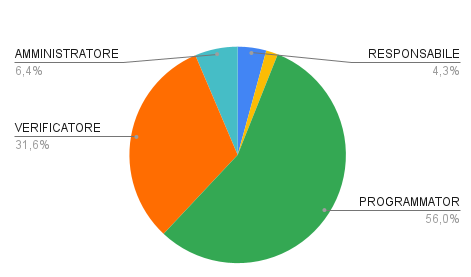
\includegraphics[width=0.6\linewidth]{grafici/11_periodo_torta.png}
  \caption{Ripartizione dei costi per ruolo nell'$11^\circ$ periodo}
        \vspace{5mm}
  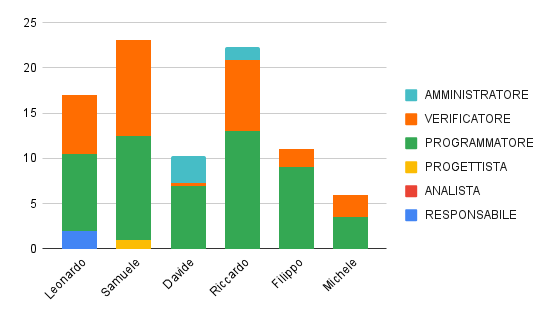
\includegraphics[width=0.7\linewidth]{grafici/11_periodo_istogramma.png}
  \caption{Ore preventivate per ciascuna persona nell'$11^\circ$ periodo}
\end{figure}
\subsubsubsection{Review}
Le attività preventivate sono state svolte con successo.
\subsubsubsubsection*{Attività svolte}
Le attività svolte in questo periodo sono state le seguenti:
\begin{itemize}
    \item Effettuato incontro con il proponente per discutere di dubbi riguardo al documento Specifica Tecnica; mostrato lo stato di avanzamento dei lavori.
    \item Effettuato incontro con il prof. Cardin per discutere di dubbi riguardanti il documento Specifica Tecnica.
\item Rivista la progettazione logica in seguito al $\textit{feedback}_G$ da parte del prof. Cardin.
\item Continuazione con la stesura del documento $\textit{Manuale Utente}_G$;
\item Completati i requisiti funzionali obbligatori;
\item Raggiunta la copertura dei $\textit{test}_G$ voluta dal proponente;
\item Implementato il $\textit{sistema}_G$ di notifica;
\item Effettuato incontro con il proponente per l'approvazione del $\textit{MVP}_G$ e ricevuta l'approvazione.
\end{itemize}
\subsubsubsubsection*{Consuntivo}
\begin{table}[H]
    \centering
\begin{spreadtab}{{tabular}{|c|c|c|c|c|c|c|c|}}
    \hline
    @\textbf{Membro} & @\textbf{Re} & @\textbf{Amm} & @\textbf{An} & @\textbf{Progr} & @\textbf{Proge} & @\textbf{Ve} & @\textbf{Totale} \\
    \hline
    @ Samuele V.   & 0          & 0          & 0         & 14          & 0.5     & 9.25     & sum(b2:g2) \\
    @ Leonardo B.  & 2.75         & 0          & 0        & 13.34        & 0     & 6.67    & sum(b3:g3) \\
    @ Riccardo Z.  & 0         & 1.5 & 0          & 14.17         & 0     & 5.83   & sum(b4:g4) \\
    @ Davide B.    & 0          & 6.75         & 0       & 11.5       & 0     & 0.5     & sum(b5:g5) \\
    @ Michele Z.   & 0          & 0          & 0         & 11.5          & 0     & 2.5     & sum(b6:g6) \\
    @ Filippo T.   & 0          & 0          & 0         & 5.5          & 0     & 0.83     & sum(b7:g7) \\
    \hline
    @\textbf{Ore totali} & sum(b2:b7) & sum(c2:c7) & sum(d2:d7) & sum(e2:e7) & sum(f2:f7) & sum(g2:g7) &  sum(b8:g8)\\
    \hline
    @\textbf{Costo totale} & 30*b8 & 20*c8 & 25*d8 & 15*e8 & 25*f8 & 15*g8 & sum(b9:g9)\\
    \hline
\end{spreadtab}
    \caption{Consuntivo orario ed economico parziale per l'undicesimo periodo, in base al ruolo}
    \label{tab:prev_rtb}
    \vspace{5mm}
    \textbf{Legenda:} \textit{Re} = Responsabile, \textit{Amm} = Amministratore, \textit{An} = Analista, \textit{Progr} = Programmatore, \textit{Proge} = Progettista, \textit{Ve} = Verificatore
\end{table}

\begin{comment}
\begin{figure}[H]
  \centering
  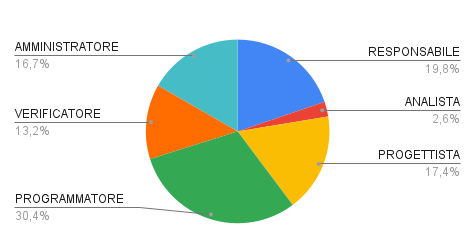
\includegraphics[width=0.6\linewidth]{grafici/10_periodo_torta.png}
  \caption{Ripartizione dei costi per ruolo nel $10^\circ$ periodo}
        \vspace{5mm}
  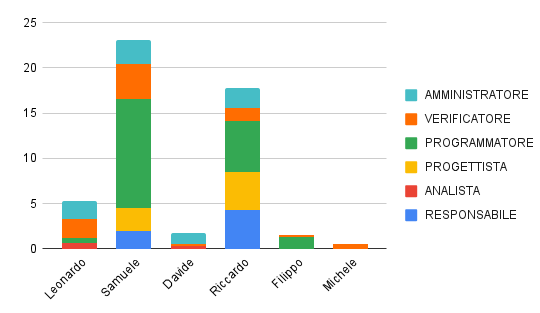
\includegraphics[width=0.7\linewidth]{grafici/10_periodo_istogramma.png}
  \caption{Ore preventivate per ciascuna persona nel $10^\circ$ periodo}
\end{figure}
\end{comment}

\begin{figure}[H]
  \centering
  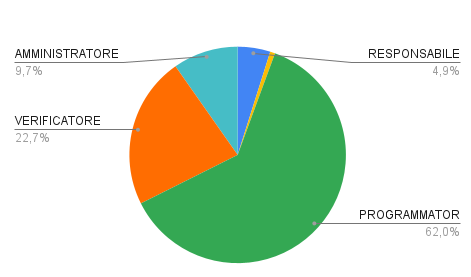
\includegraphics[width=0.6\linewidth]{grafici/11_periodo_torta_consuntivo.png}
  \caption{Consuntivo della ripartizione dei costi per ruolo nell'$11^\circ$ periodo}
        \vspace{5mm}
  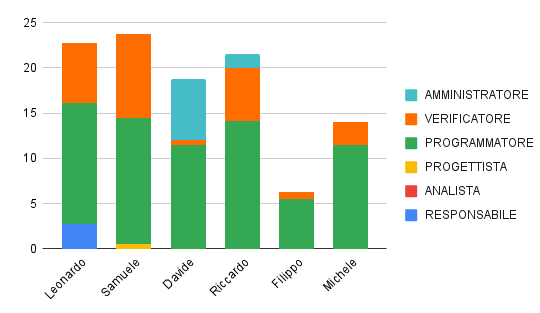
\includegraphics[width=0.7\linewidth]{grafici/11_periodo_instogramma_consuntivo.png}
  \caption{Ore eseguite per ciascuna persona nell'$11^\circ$ periodo}
\end{figure}

\subsubsubsection{Retrospective}
\paragraph*{Gestione dei Rischi}
I $\textit{rischi}_G$ affrontati durante questo periodo sono stati i seguenti:
\begin{itemize}
\item \nameref{ro:2}: la limitata disponibilità di alcuni membri del team ha determinato un rallentamento previsto nello $\textit{sprint}_G$.
\begin{itemize}
\item \textbf{Esito della mitigazione}: una redistribuzione di alcune attività ha comunque permesso di completare lo $\textit{sprint}_G$ e implementare tutte le funzionalità rimanenti.
\item \textbf{Impatto}: La redistribuzione ha causato un maggiore squilibrio nelle ore individuali lavorate dai membri del gruppo.
\end{itemize}
\item \nameref{ro:5}: la scarsa esperienza nella progettazione e nel testing ha comportato un rallentamento previsto nello $\textit{sprint}_G$.
\begin{itemize}
\item \textbf{Esito della mitigazione}: le attività di studio individuale, le discussioni di gruppo e gli incontri frequenti con il proponente e il prof. Cardin sono stati elementi chiave per mitigare questo rischio. In particolare, per ogni risultato ottenuto in fase di testing e progettazione, è stata fornita una dimostrazione al proponente, ottenendo un riscontro tempestivo; i progressi nella stesura del documento Specifica Tecnica sono stati mostrati al prof. Cardin, che ha fornito $\textit{feedback}_G$ al gruppo.
\item \textbf{Impatto}: in ambito progettuale, sono stati chiariti alcuni dubbi relativi al documento Specifica Tecnica.
\end{itemize}
\end{itemize}
\paragraph*{Considerazioni e pianificazione futura}
\begin{itemize}
    \item L'incontro con il prof. Cardin ha evidenziato i problemi dell'$\textit{architettura}_G$ logica del prodotto. Infatti il gruppo ha compreso che si doveva modificare l'$\textit{architettura}_G$ logica suddividendola da quella di $\textit{deployment}_G$.
    \item Nel periodo successivo si dovrà sistemare il documento di Specifica Tecnica per sostenere la revisione $\textit{PB}_G$ con il prof. Cardin.
\end{itemize}
 
\newpage

% Undicesimo periodo
\subsubsection{Dodicesimo periodo (2024/05/30 - 2024/06/11)}
\subsubsubsection{Planning}
In questo ultimo periodo il gruppo si propone come obiettivo quello di completare tutta la documentazione in vista dell'ultima revisione. Si è quindi pianificato di scrivere una mail al prof. Cardin per fissare una data per effettuare la revisione $\textit{PB}_G$. Nel mentre, il gruppo prevede di sistemare i vari documenti per l'incontro col prof. Vardanega, cercando quindi di ottimizzare i tempi per fissare poi una data per l'interrogazione il prima possibile.
\subsubsubsubsection*{Attività pianificate}
Gli obiettivi posti per lo $\textit{sprint}_G$ sono stati i seguenti:
\begin{itemize}
    \item Effettuare il colloquio con il prof. Cardin per la revisione $\textit{PB}_G$ in data 5 giugno, per il quale si vuole:
    \begin{itemize}
        \item Preparare le diapositive per il colloquio;
        \item Preparare la lettera di presentazione per la fase $\textit{PB}_G$.
    \end{itemize}
    \item Redigere il $\textit{manuale utente}_G$;
    \item Aggiornare il documento di Analisi dei Requisiti;
    \item Aggiornare il documento $\textit{Piano di Qualifica}_G$;
    \item Aggiornare il documento $\textit{Norme di Progetto}_G$;
    \item Aggiornare il documento $\textit{Piano di Progetto}_G$;
    \item Aggiornare il documento Glossario Tecnico;
    \item Approvare tutti i documenti in vista dell'interrogazione col prof. Vardanega.
\end{itemize}
\subsubsubsubsection*{Preventivo}
\begin{table}[H]
    \centering
\begin{spreadtab}{{tabular}{|c|c|c|c|c|c|c|c|}}
    \hline
    @\textbf{Membro} & @\textbf{Re} & @\textbf{Amm} & @\textbf{An} & @\textbf{Progr} & @\textbf{Proge} & @\textbf{Ve} & @\textbf{Totale} \\
    \hline
    @ Samuele V.   & 0         & 0         & 0         & 0        & 6.5   & 1     & sum(b2:g2) \\
    @ Leonardo B.  & 2         & 3.5       & 0         & 3        & 8     & 2     & sum(b3:g3) \\
    @ Riccardo Z.  & 0         & 2         & 0         & 0        & 1     & 1     & sum(b4:g4) \\
    @ Davide B.    & 3         & 7.5       & 1         & 2.5      & 5     & 3     & sum(b5:g5) \\
    @ Michele Z.   & 3.5       & 3         & 0         & 5        & 4.5   & 8     & sum(b6:g6) \\
    @ Filippo T.   & 5.75      & 10        & 0         & 5.5      & 3.5   & 6.5   & sum(b7:g7) \\
    \hline
    @\textbf{Ore totali} & sum(b2:b7) & sum(c2:c7) & sum(d2:d7) & sum(e2:e7) & sum(f2:f7) & sum(g2:g7) &  sum(b8:g8)\\
    \hline
    @\textbf{Costo totale} & 30*b8 & 20*c8 & 25*d8 & 15*e8 & 25*f8 & 15*g8 & sum(b9:g9)\\
    \hline
\end{spreadtab}
    \caption{Preventivo orario ed economico parziale per il dodicesimo periodo, in base al ruolo}
    \vspace{5mm}
    \textbf{Legenda:} \textit{Re} = Responsabile, \textit{Amm} = Amministratore, \textit{An} = Analista, \textit{Progr} = Programmatore, \textit{Proge} = Progettista, \textit{Ve} = Verificatore
\end{table}
\begin{figure}[H]
    \centering
    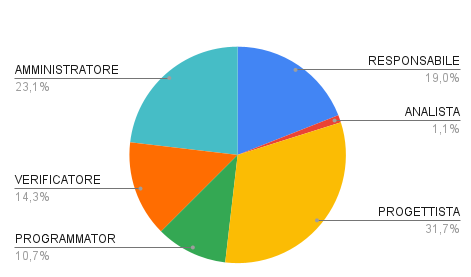
\includegraphics[width=0.6\linewidth]{grafici/12_periodo_torta.png}
    \caption{Ripartizione dei costi per ruolo nell'$12^\circ$ periodo}
        \vspace{5mm}
    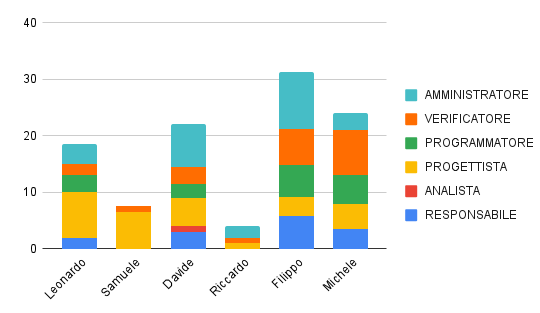
\includegraphics[width=0.7\linewidth]{grafici/12_periodo_istogramma.png}
    \caption{Ore preventivate per ciascuna persona nell'$12^\circ$ periodo}
\end{figure}
\subsubsubsection{Review}
Le attività preventivate sono state svolte con successo. La stesura e approvazione dei documenti ha richiesto più tempo di quanto sperato, nonostante ciò i tempi rientrano nelle previsioni.
\subsubsubsubsection*{Attività svolte}
Le attività svolte in questo periodo sono state le seguenti:
\begin{itemize}
    \item Effettuato l'incontro col prof. Cardin;
    \item Redatto e approvato il documento $\textit{Manuale Utente}_G$;
    \item Aggiornato e approvato il documento Analisi dei Requisiti;
    \item Aggiornato e approvato il documento $\textit{Piano di Qualifica}_G$;
    \item Aggiornato e approvato il documento $\textit{Norme di Progetto}_G$;
    \item Aggiornato e approvato il documento Glossario Tecnico;
    \item Aggiornato e approvato il documento $\textit{Piano di Progetto}_G$;
    \item Redigere la lettera di presentazione $\textit{PB}_G$ riservata alla seconda parte della revisione.
\end{itemize}

\subsubsubsubsection*{Consuntivo}
\begin{table}[H]
    \centering
\begin{spreadtab}{{tabular}{|c|c|c|c|c|c|c|c|}}
    \hline
    @\textbf{Membro} & @\textbf{Re} & @\textbf{Amm} & @\textbf{An} & @\textbf{Progr} & @\textbf{Proge} & @\textbf{Ve} & @\textbf{Totale} \\
    \hline
    @ Samuele V.   & 0        & 0         & 0         & 0         & 2.59  & 0.14  & sum(b2:g2) \\
    @ Leonardo B.  & 1.25     & 1.25      & 0         & 4         & 9.75  & 1     & sum(b3:g3) \\
    @ Riccardo Z.  & 0        & 1         & 0         & 0         & 0.5   & 0.5   & sum(b4:g4) \\
    @ Davide B.    & 3        & 8         & 1         & 2.5       & 5     & 3     & sum(b5:g5) \\
    @ Michele Z.   & 3.5      & 3.5       & 0         & 7         & 5.5   & 3.5   & sum(b6:g6) \\
    @ Filippo T.   & 6.75     & 12        & 0         & 7.75      & 2.83  & 12    & sum(b7:g7) \\
    \hline
    @\textbf{Ore totali} & sum(b2:b7) & sum(c2:c7) & sum(d2:d7) & sum(e2:e7) & sum(f2:f7) & sum(g2:g7) &  sum(b8:g8)\\
    \hline
    @\textbf{Costo totale} & 30*b8 & 20*c8 & 25*d8 & 15*e8 & 25*f8 & 15*g8 & sum(b9:g9)\\
    \hline
\end{spreadtab}
    \caption{Consuntivo orario ed economico parziale per il dodicesimo periodo, in base al ruolo}
    \vspace{5mm}
    \textbf{Legenda:} \textit{Re} = Responsabile, \textit{Amm} = Amministratore, \textit{An} = Analista, \textit{Progr} = Programmatore, \textit{Proge} = Progettista, \textit{Ve} = Verificatore
\end{table}
\begin{figure}[H]
    \centering
    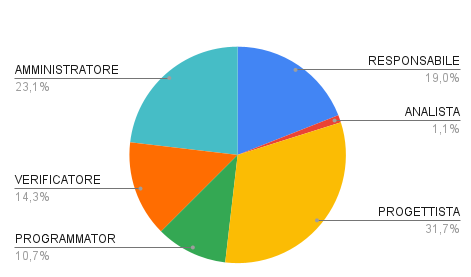
\includegraphics[width=0.6\linewidth]{grafici/12_periodo_torta_consuntivo.png}
    \caption{Consuntivo della ripartizione dei costi per ruolo nell'$12^\circ$ periodo}
        \vspace{5mm}
    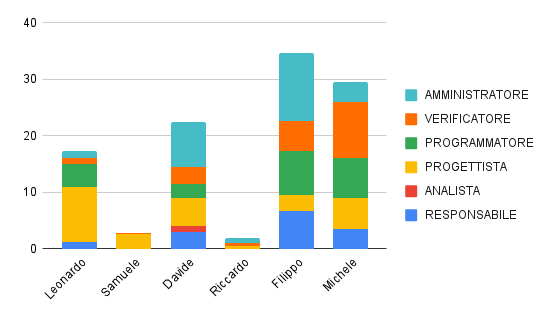
\includegraphics[width=0.7\linewidth]{grafici/12_periodo_istogramma_consuntivo.png}
    \caption{Ore eseguite per ciascuna persona nell'$12^\circ$ periodo}
\end{figure}
\subsubsubsection{Retrospective}
\paragraph*{Gestione dei Rischi}
I $\textit{rischi}_G$ occorsi per tale periodo sono stati i seguenti:
\begin{itemize}
    \item \nameref{ro:3}: Alcuni membri del gruppo, hanno avuto difficoltà a svolgere alcune task per tempo, a causa di impegni personali.
    \begin{itemize}
        \item \textbf{Esito mitigazione}: la possibilità che tale evento potesse accadere era stata notificata con anticipo, quindi si era già messo in conto un possibile ritardo nel completamento delle attività.
        \item \textbf{Impatto}: I tempi di completamento delle tasks si sono allungati, in particolar modo ha ritardato lo svolgimento di task di verifica, riguardanti documenti non ancora aggiornati.
    \end{itemize}
    \item \nameref{ro:5}: Alcuni membri del gruppo avevano da redigere documenti con cui avevano poca familiarità.
    \begin{itemize}
        \item \textbf{Esito mitigazione}: qualora qualche membro del gruppo avesse avuto difficoltà a redigere o verificare qualche documento, i membri del gruppo più liberi ed esperti erano disposti a dare una mano.
        \item \textbf{Impatto}: I tempi di completamento si sono comunque allungati un po', ma nel complesso non c'è stato un impatto negativo.
    \end{itemize}
\end{itemize}
\paragraph*{Considerazioni}
\begin{itemize}
    \item Nonostante i leggeri ritardi nell'esecuzione delle varie tasks, il gruppo è soddisfatto dei tempi di completamento degli obiettivi fissati per questo periodo.
\end{itemize}